\chapter{Applications} \label{ch:applications}

Everything so far has been either machinery or a model. This chapter is the place where both are
made to meet market data. Three studies are carried out. The first two calibrate the same index on
the same value date and are deliberately complementary; the third is not a calibration at all, and
measures the underlying series directly.


The first fits an implied volatility surface directly, imposing the static no-arbitrage conditions of
Proposition \ref{prop:staticarbitrage} as penalties rather than inheriting them from a parametric
family, and extrapolating beyond the quoted range by a closed form on which those conditions are
\emph{proved} rather than sampled. The second fits that index with the rough Heston model of
Definition \ref{def:roughheston}, so that a model with dynamics --- and with the short-dated skew
that Chapter \ref{ch:roughpaths} identified as the empirical signature of roughness --- is measured
against a surface fitted with no dynamics at all. Section \ref{sec:pinn} produces the best possible \emph{description} of
today's option prices; Section \ref{sec:roughcalib} produces the best possible \emph{explanation} of
them within a two-factor rough model. 

The third study, Section \ref{sec:levyresults}, changes both the data and the question. It leaves
the option book entirely and works on eleven years of daily closes of two equity indices, computing
the level-two signature of the resulting planar path. This is the one place in the thesis where the
machinery of Chapter \ref{ch:roughpaths} is used as machinery rather than as vocabulary: the objects
evaluated are the L\'evy area and Chen's relation themselves, the identities they satisfy are checked
as identities, and the estimator built from them in Subsection \ref{subsec:levyarea} is read on real
data and then deliberately tested against a case whose answer is known in advance.

\begin{notationbox}[Symbols of this chapter]\label{not:applications}
The surface conventions of Chapter \ref{ch:finance} are kept without exception: $\lmon =
\log(\Strike/\Fwd(t,T))$ is log-moneyness, $T$ is the maturity coordinate, $\ivol(\lmon,T)$ is the
implied volatility, $\tvar = \ivol^{2}T$ the total implied variance and $\lvol$ the local
volatility. Two derived quantities recur throughout and are fixed here: the \textbf{normalised
skew} $\nskew := \lmon\,\ivd{k}/\ivol$, and the \textbf{log-elasticity} in maturity
$\elas{f} := \partial\log f/\partial\log T$, used as $\elas{\ivol}$ and $\elas{\tvar}$.
\end{notationbox}

%===========================================================================
\section{Calibration of an Implied Volatility Surface with a PINN}
\label{sec:pinn}

Subsection \ref{subsec:localvol} established that local volatility is the unique diffusion
reproducing a given arbitrage-free implied volatility surface, and the route is Dupire's
formula \eqref{eq:dupire}:
\begin{equation}\label{eq:gatheralrecall}
  \lvol^{2}(\lmon,T) \;=\; \frac{\partial_{T}\tvar}{g},
\end{equation}
whose denominator is exactly the butterfly quantity $g$ of \eqref{eq:butterfly} and whose numerator
is exactly the calendar quantity \eqref{eq:calendarspread}. The whole of this section is an attempt
to build a surface for which the right-hand side of \eqref{eq:gatheralrecall} is well defined
everywhere, including where nothing is quoted.

The classical response is to fit a parametric slice model --- SVI \cite{gatheral2014} and its
descendants --- maturity by maturity, and then to repair the slices so that they do not cross. We
take a different route. We construct a single globally smooth function of $(\lmon,T)$, represented by
a small neural network in the region where the market quotes and by a closed-form asymptotic family
outside it, and we impose the two conditions of Proposition \ref{prop:staticarbitrage} as penalties
evaluated at collocation points during training. This is the \emph{physics-informed neural network}
(PINN) methodology of Raissi, Perdikaris and Karniadakis \cite{raissi2019}, applied not to a PDE
residual but to a pair of differential inequalities.

Neural representations of the implied volatility surface carrying no-arbitrage penalties are not
new. Ackerer, Tagasovska and Vatter \cite{ackerer2020} smooth the surface with a network trained
under soft arbitrage constraints, and Chataigner, Cr\'epey and Dixon \cite{chataigner2020} do the
same with the local volatility as the target. What is added here is confined to the extrapolated
region: the wings are not learned at all but given in closed form, the no-arbitrage conditions are
\emph{proved} on them (Lemma \ref{lem:master} and Theorem \ref{thm:wingreduction}) rather than
sampled at collocation points, and they are joined to the network with $C^{3}$ continuity.

A full account of PINNs, of their capabilities and of their limitations, is outside the scope of this
dissertation; the reader interested in these approaches to numerical problems is referred to
\cite{raissi2019} and to the survey \cite{karniadakis2021}. We record only that they have been
successful on direct and inverse problems in disciplines --- fluid dynamics above all --- where
classical approaches are hard, and that for our purposes the decisive feature is a narrow one:
automatic differentiation \cite{baydin2018} supplies derivatives of the represented function that
are exact up to machine precision. A condition such as $g\ge0$, which is a statement about
$\ivd{k}$ and $\ivd{kk}$, can therefore be evaluated at a point rather than estimated from a
difference quotient.

The distinguishing features of the construction, relative to a naive PINN, are the following.

\begin{enumerate}
  \item The asymptotic behaviour is \emph{not learned}. Beyond a fixed attachment point on each side
    the surface is an explicit saturating exponential whose three parameters are read off the
    network's own local jet and then projected onto a region where the conditions of Proposition
     \ref{prop:staticarbitrage} hold \emph{identically}. 
     %Extrapolation is therefore a theorem, not an
    % extrapolation.
  \item The surface is $C^{3}$ across every internal frontier by construction, so by
    \eqref{eq:gatheralrecall} the local volatility is $C^{1}$ and can itself be differentiated.
  \item No derivative appearing in the loss is a finite difference in $\lmon$. All
    $\lmon$-derivatives are exact, obtained by forward-mode propagation of a truncated jet through
    the network.
  \item The calendar condition on the extrapolated wings is reduced, by an exact minimisation, to
    three scalar monotonicity statements in $T$ (Theorem \ref{thm:wingreduction}).
\end{enumerate}

% We develop these in turn.

% % ---------------------------------------------------------------------------
% \subsection{No-Arbitrage in Volatility Coordinates}
% \label{subsec:volcoords}

Proposition \ref{prop:staticarbitrage} is stated in total-variance coordinates because that is where
the conditions are cleanest. The object we shall parameterise, however, is $\ivol$ itself: it is what
is quoted, what carries a bid--ask spread, and what has a bounded and well-conditioned range across
the whole surface, whereas $\tvar$ varies by two orders of magnitude between one month and five
years. The following elementary translation is therefore the bridge between the theory of Chapter
\ref{ch:finance} and the model of this section, and it is used at every collocation point.

\begin{proposition}[The butterfly quantity in volatility coordinates]\label{prop:gvol}
Let $\ivol(\lmon,T)>0$ be twice differentiable in $\lmon$ and set $\tvar=\ivol^{2}T$. Then the
function $g$ of \eqref{eq:butterfly} satisfies
\begin{equation}\label{eq:gvol}
  g \;=\; \bigl(1-\nskew\bigr)^{2}\;-\;\tfrac{1}{4}\,T^{2}\ivol^{2}\,\ivd{k}^{2}\;+\;T\,\ivol\,\ivd{kk},
  \qquad \nskew=\frac{\lmon\,\ivd{k}}{\ivol},
\end{equation}
and the calendar quantity satisfies
\begin{equation}\label{eq:calvol}
  \partial_{T}\tvar \;=\; \ivol^{2}\bigl(1+2\,\elas{\ivol}\bigr),
  \qquad
  \elas{\ivol}=\frac{T\,\ivd{T}}{\ivol}, \qquad 1+2\elas{\ivol}=\elas{\tvar} .
\end{equation}
\end{proposition}

\textbf{\textit{Proof:}} From $\tvar=\ivol^{2}T$ we get $\partial_{\lmon}\tvar=2T\ivol\,\ivd{k}$ and
$\partial^{2}_{\lmon\lmon}\tvar=2T\bigl(\ivd{k}^{2}+\ivol\,\ivd{kk}\bigr)$. Substituting into
\eqref{eq:butterfly} term by term, the first term is
\[
  \Bigl(1-\frac{\lmon\,\partial_{\lmon}\tvar}{2\tvar}\Bigr)^{2}
  =\Bigl(1-\frac{\lmon\cdot 2T\ivol\,\ivd{k}}{2T\ivol^{2}}\Bigr)^{2}=(1-\nskew)^{2},
\]
the second is
\[
  -\frac{(\partial_{\lmon}\tvar)^{2}}{4}\Bigl(\frac{1}{\tvar}+\frac14\Bigr)
  =-T^{2}\ivol^{2}\ivd{k}^{2}\Bigl(\frac{1}{T\ivol^{2}}+\frac14\Bigr)
  =-T\,\ivd{k}^{2}-\tfrac14 T^{2}\ivol^{2}\ivd{k}^{2},
\]
and the third is $\tfrac12\partial^{2}_{\lmon\lmon}\tvar=T\ivd{k}^{2}+T\ivol\,\ivd{kk}$. The two
occurrences of $T\,\ivd{k}^{2}$ cancel, which leaves \eqref{eq:gvol}. For \eqref{eq:calvol},
$\partial_{T}\tvar=\partial_{T}(\ivol^{2}T)=\ivol^{2}+2T\ivol\,\ivd{T}=\ivol^{2}(1+2\elas{\ivol})$,
and dividing by $\tvar/T=\ivol^{2}$ gives $T\partial_T\tvar/\tvar=\elas{\tvar}=1+2\elas{\ivol}$.
\qedfilledtext

\medskip

The cancellation is what makes the volatility parameterisation
workable at all. In \eqref{eq:butterfly} the slope enters through two terms of opposite sign whose
leading parts are both $O(T)$; in \eqref{eq:gvol} that part is gone and what survives is a clean
decomposition
\begin{equation}\label{eq:gsplit}
  g \;=\; g_{\mathrm{slope}}+T\,\ivol\,\ivd{kk},
  \qquad
  g_{\mathrm{slope}}:=(1-\nskew)^{2}-\tfrac14T^{2}\ivol^{2}\ivd{k}^{2},
\end{equation}
in which the curvature appears exactly once, linearly, and with a positive sign. Two consequences
follow immediately, and both shape the objective of \S\ref{subsec:objective}.

\begin{proposition}[Qualitative behaviour with short maturities]\label{prop:shortdated}
Suppose $\ivol$, $\ivd{k}$ and $\ivd{kk}$ remain bounded as $T\downarrow0$, and work on the branch
$\nskew<1$. Both correction terms in \eqref{eq:gvol} carry explicit positive powers of $T$, so
$g\to(1-\nskew)^{2}$ as $T\to0^{+}$, and a margin $g\ge g_{\star}$ maintained in that limit forces
\begin{equation}\label{eq:shortdatedbound}
  \nskew \;\le\; 1-\sqrt{g_{\star}},
\end{equation}
irrespective of the curvature. This is a statement about the limit, not a constraint imposed exactly
at each individual small maturity.
\end{proposition}

\textbf{\textit{Proof:}}
Immediate from \eqref{eq:gvol}, the two correction terms being $O(T^{2})$ and $O(T)$ with $\ivol$,
$\ivd{k}$, $\ivd{kk}$ bounded. At $T=0$ the requirement reads $(1-\nskew)^{2}\ge g_{\star}$, so that on
the branch $\nskew<1$ this is
\eqref{eq:shortdatedbound}. \qedfilledtext

\begin{remark}[The curvature enters linearly and benignly]\label{prop:curvlinear}
In \eqref{eq:gsplit} the curvature term $T\ivol\,\ivd{kk}$ is linear in $\ivd{kk}$ with a
\emph{positive} coefficient. Consequently:
\begin{itemize}
  \item[i)] a given change of slope spread over $m$ times the width costs $1/m$ of the density; in
    particular, spreading it over three times the width recovers two thirds of the cost;
  \item[ii)] positive curvature \emph{raises} $g$, so curvature is a cost only where it is
    negative --- and that is precisely the case of interest here, since a rising wing approaching a
    finite asymptote must approach it concavely. At the join this is $\ivd{kk}=-s/\ell<0$ by
    \eqref{eq:wingjet},
    which is what \eqref{eq:joinbutterfly} charges for and what forces the floor
    \eqref{eq:ellmin} on $\ell$.
\end{itemize}
\end{remark}

% \begin{proof}
% Both parts are read off the linearity. For i), a slope change $\delta$ effected over an interval of
% width $L$ has mean curvature $\ivd{kk}\simeq\delta/L$, so replacing $L$ by $mL$ multiplies
% $T\ivol\,\ivd{kk}$ by $1/m$; when $\delta<0$, which is the case that costs density, the shortfall
% $|T\ivol\,\ivd{kk}|$ is divided by $m$ and a fraction $1-1/m$ of it is recovered. For ii), if
% $\ivd{kk}\ge0$ then $T\ivol\,\ivd{kk}\ge0$ and $g\ge g_{\mathrm{slope}}$.
% \end{proof}

% Proposition \ref{prop:shortdated} explains why no amount of curvature penalty can repair a
% short-dated smile whose skew is too steep; the model instead damps $\nskew$ directly. Proposition
% \ref{prop:curvlinear} is the reason the wing shape penalties described in \S\ref{subsec:shape} are
% one-sided in the sign of $\ivd{kk}$: a symmetric version penalises exactly the benign case ii).

% ---------------------------------------------------------------------------
% \subsection{The Model}
% \label{subsec:the-model}

\subsubsection*{Inputs}

The only inputs the model requires are implied volatility observations with the strike and maturity
they belong to, $(T,\Strike/\Fwd,\ivol)$. Observations sharing a $(T,\Strike)$ are grouped into a
single quote, the bid and ask being the smallest and largest of the group and the mid their mean; a
lone observation is given a half-spread of one basis point. The band is therefore the true bid/ask,
and $h$ in \eqref{eq:fitresidual} is half of it.
This implicitly hides one preliminary step, namely the forward curve calibration needed to invert the
volatilities out of market prices through Definition \ref{def:impliedvol}, the forward being the
one fixed in Definition \ref{def:forwardprice}. We assume throughout that this has been done.

The quotes used in this chapter are consensus mid, bid and ask implied volatilities for S\&P 500
index options, for the value date 3 March 2025, obtained from the Totem service of S\&P Global
Market Intelligence \cite{totem}, a monthly consensus pricing platform for over-the-counter
derivatives. Totem quotes are contributed and are therefore European in style and quoted on a fixed
moneyness grid rather than on a listed strike ladder, which is why the maturities reach well beyond
the horizon of exchange-listed contracts. Access is restricted to contributing institutions, so the
data cannot be redistributed with this dissertation; the same source has been used in the academic
literature, for instance by Ergun and Uthemann \cite{ergunuthemann2020}. What follows deals with the volatility surface alone.

\subsubsection*{The functional form}

Fix two attachment points $\lmon^{*}_{\mathrm{L}}<0<\lmon^{*}_{\mathrm{R}}$ and two collar widths
$\Lambda_{\mathrm{L}},\Lambda_{\mathrm{R}}>0$, and introduce on each side the \emph{outward
coordinate}
\begin{equation}\label{eq:outward}
  x_{\mathrm{L}}(\lmon)=\lmon^{*}_{\mathrm{L}}-\lmon,
  \qquad
  x_{\mathrm{R}}(\lmon)=\lmon-\lmon^{*}_{\mathrm{R}},
\end{equation}
so that $x_{\mathrm{s}}>0$ is the extrapolation region on that side and $x_{\mathrm{s}}<0$ points
back into the quoted range. The surface is
\begin{equation}
  \boxed{\;
  \ivol(\lmon,T)\;=\;\Core(\lmon,T)\;+\;\sum_{\mathrm{s}\in\{\mathrm{L},\mathrm{R}\}}
    \Bigl(\Wing_{\mathrm{s}}(\lmon,T)-\Core(\lmon,T)\Bigr)\,\Psi\!\left(z_{\mathrm{s}}(\lmon)\right)
  \;}
  \label{eq:surface}
\end{equation}
where
\begin{itemize}
  \item $\Core$ is a small multilayer perceptron with parameters $\Theta$, positive by construction
    (\S\ref{subsec:network});
  \item $\Wing_{\mathrm{s}}$ is the analytic wing,
    \begin{equation}
      \Wing_{\mathrm{s}}(\lmon,T)\;=\;a(T)\;+\;b(T)\Bigl(1-e^{-x_{\mathrm{s}}(\lmon)/\ell(T)}\Bigr),
      \label{eq:wing}
    \end{equation}
    with level $a>0$, saturation length $\ell>0$ and lift $b$ of either sign, one such triple per
    side;
  \item $\Psi$ is a smooth cut-off supported on the collar: with
    \begin{equation}\label{eq:collarcoord}
      z_{\mathrm{s}}(\lmon)\;=\;\min\Bigl\{1,\;\max\Bigl\{0,\;-\tfrac{x_{\mathrm{s}}(\lmon)}{\Lambda_{\mathrm{s}}}\Bigr\}\Bigr\}\in[0,1],
    \end{equation}
    $\Psi$ satisfies $\Psi(0)=1$ and $\Psi(1)=0$, and is specified in \S\ref{subsec:smoothness}.
\end{itemize}

The clamp in \eqref{eq:collarcoord} is what makes \eqref{eq:surface} a single expression rather than
a case distinction. For $x_{\mathrm{s}}>0$ we have $z_{\mathrm{s}}=0$ and $\Psi=1$, so
$\ivol\equiv\Wing_{\mathrm{s}}$: the tail is the blend evaluated at its own endpoint, not a separate
branch. For $x_{\mathrm{s}}<-\Lambda_{\mathrm{s}}$ we have $z_{\mathrm{s}}=1$, $\Psi=0$ and
$\ivol\equiv\Core$. In between, the two are blended. One formula, three regimes.

\begin{remark}
The two collars never overlap in practice, and the implementation caps
$\Lambda_{\mathrm{L}}+\Lambda_{\mathrm{R}}$ at a fixed fraction of
$\lmon^{*}_{\mathrm{R}}-\lmon^{*}_{\mathrm{L}}$. Where they did overlap, \eqref{eq:surface} would
still be well defined but the interpretation as ``one wing at a time'' would fail.
\end{remark}

\subsubsection*{What is imposed}

By Proposition \ref{prop:staticarbitrage} and Proposition \ref{prop:gvol}, absence of static
arbitrage is secured by the two inequalities
\begin{equation}\label{eq:twoconditions}
  g\;\ge\;0
  \qquad\text{and}\qquad
  \partial_{T}\tvar\;=\;\ivol^{2}\bigl(1+2\elas{\ivol}\bigr)\;\ge\;0 ,
\end{equation}
with $g$ given by \eqref{eq:gvol}, the third condition of that proposition --- Lee's wing bound
\cite{lee2004} --- being automatic for \eqref{eq:wing}, as noted in \S\ref{subsec:wings}. In practice
both are imposed with a strictly positive margin: $g\ge g_{\star}$ and $\elas{\tvar}\ge c_{\star}$
with $g_{\star},c_{\star}>0$. The reason is stated once here and used throughout. A surface satisfying
$g\ge0$ with equality attained is one on which the risk-neutral density of Proposition
\ref{prop:breedenlitzenberger} vanishes, and by \eqref{eq:gatheralrecall} the local variance there is
infinite; a margin is what keeps \eqref{eq:gatheralrecall} usable rather than merely non-negative.

% ---------------------------------------------------------------------------
\subsection{The Analytic Wings}
\label{subsec:wings}

 Nothing in the architecture prevents a fitted surface from turning over at $|\lmon|=3$, and
Lee's moment formula \cite{lee2004} is a statement about a limit, not
a penalty one can evaluate at a finite collocation point. We therefore replace the network by the
three-parameter family \eqref{eq:wing} beyond $\lmon^{*}$ and \emph{prove} the two conditions
\eqref{eq:twoconditions} on that family.

Write the wing in terms of its jet at the join. Dropping the side subscript, with $a=\Wing(0)$ the
level, $s=\ivd{x}(0)$ the outward slope and $\ell$ the saturation length,
\begin{equation}\label{eq:wingjet}
  b=s\,\ell,\qquad \ivd{x}(x)=s\,e^{-x/\ell},\qquad \ivd{xx}(x)=-\tfrac{s}{\ell}\,e^{-x/\ell},
  \qquad \Winf=a+b .
\end{equation}
It is convenient to use $\tvar_{0}=T a^{2}$, the total variance at the join, and the dimensionless
slope
\begin{equation}\label{eq:sjoin}
  \nskew_{0}\;=\;\frac{|\lmon^{*}|\,s}{a},
\end{equation}
which is the normalised skew $\nskew$ of Notation \ref{not:applications} evaluated at the join, on
either side: at $x=0$ we have $\lmon=\lmon^{*}$, $\ivol=a$ and $\lmon\,\ivd{k}=|\lmon^{*}|s$, the
signs cancelling on the left wing. Two structural facts are immediate and carry no loss
weight:
\begin{itemize}
  \item $\ivd{x}=s\,e^{-x/\ell}$ never vanishes unless $b=0$, so the surface has \emph{no extremum}
    beyond $\lmon^{*}$;
  \item $\ivol\to\Winf$, so $\tvar\sim\Winf^{2}T$ is bounded in $\lmon$ and condition iii) of
    Proposition \ref{prop:staticarbitrage} holds with room to spare.
\end{itemize}

\subsubsection*{The butterfly condition at the join}

Substituting \eqref{eq:wingjet} into $g\ge g_{\star}$ at $x=0$, using
$\ivd{k}^{2}=s^{2}$ and $\ivd{kk}=-s/\ell$ and eliminating $s$ through \eqref{eq:sjoin}, gives
\begin{equation}
  (1-\nskew_{0})^{2}\;-\;\frac{\tvar_{0}^{2}\nskew_{0}^{2}}{4\lmon^{*2}}\;-\;\frac{\tvar_{0}\nskew_{0}}{|\lmon^{*}|\,\ell}
  \;\ge\;g_{\star} .
  \label{eq:joinbutterfly}
\end{equation}

On a \emph{rising} wing ($\nskew_{0}>0$) the last term is a cost, so \eqref{eq:joinbutterfly} is a
\emph{lower} bound on $\ell$, namely
\begin{equation}\label{eq:ellmin}
  \ell\;\ge\;\ell_{\min}:=\frac{\tvar_{0}\nskew_{0}/|\lmon^{*}|}
  {(1-\nskew_{0})^{2}-g_{\star}-\bigl(\tvar_{0}\nskew_{0}/2|\lmon^{*}|\bigr)^{2}} .
\end{equation}
Lemma \ref{lem:master} below requires $\ell\le c_{\ell}|\lmon^{*}|$ with $c_{\ell}\le1$, so the
admissible window in $\ell$ is non-empty precisely when $\nskew_{0}$ does not exceed a critical
value. Imposing \eqref{eq:joinbutterfly} at the worst admissible length $\ell=c_{\ell}|\lmon^{*}|$ and
multiplying through by $c_{\ell}\lmon^{*2}$ turns it into the quadratic
\begin{equation}\label{eq:phiquadratic}
  (A_{\ell}-B_{\ell})\,\nskew_{0}^{2}-(2A_{\ell}+\tvar_{0})\,\nskew_{0}+A_{\ell}(1-g_{\star})\;\ge\;0,
  \qquad A_{\ell}=c_{\ell}\lmon^{*2},\quad B_{\ell}=\tfrac14 c_{\ell}\tvar_{0}^{2},
\end{equation}
whose relevant root, rationalised, is
\begin{equation}
  \nskew_{0}^{\dagger}
  \;=\;\frac{2A_{\ell}(1-g_{\star})}
            {(2A_{\ell}+\tvar_{0})+\sqrt{\,4A_{\ell}^{2}g_{\star}+4A_{\ell}\tvar_{0}+\tvar_{0}^{2}+4A_{\ell}B_{\ell}(1-g_{\star})\,}} .
  \label{eq:phidagger}
\end{equation}

Three properties of \eqref{eq:phidagger} deserve comment.
\begin{enumerate}
  % \item The denominator is a sum of positive terms. The textbook form
  %   $(-B\pm\sqrt{\cdot})/2A$ has leading coefficient $A_{\ell}-B_{\ell}$, which passes through zero
  %   at $\tvar_{0}=2|\lmon^{*}|$ and is therefore an artificial singularity of the \emph{formula}
  %   rather than of the problem.
  \item It returns the correct root in \emph{both} orientations. For $\tvar_{0}<2|\lmon^{*}|$ the
    quadratic \eqref{eq:phiquadratic} opens upward and the feasible set is
    $[0,r_{\mathrm{small}}]$; for $\tvar_{0}>2|\lmon^{*}|$ it opens downward and the set is
    $[r_{-},r_{\mathrm{large}}]$. In both cases \eqref{eq:phidagger} returns the binding endpoint,
    and at $\tvar_{0}=2|\lmon^{*}|$, where that coefficient vanishes and the textbook form divides by
    zero, it returns the root of the surviving linear equation.
  \item At $T=0$ it reduces exactly to $1-\sqrt{g_{\star}}$ (Proposition
    \ref{prop:shortdated}). Indeed $\tvar_{0}=Ta^{2}\to0$ forces $B_{\ell}\to0$, whence the radicand
    tends to $4A_{\ell}^{2}g_{\star}$ and
    $\nskew_{0}^{\dagger}\to\frac{2A_{\ell}(1-g_{\star})}{2A_{\ell}(1+\sqrt{g_{\star}})}=1-\sqrt{g_{\star}}$.
    % The origin is an ordinary point of the formula: everything enters through $\tvar_{0}$
    % polynomially and nothing is divided by $T$.
  \item The root is always real. Every one of the four terms of the radicand is non-negative, since
    $A_{\ell},B_{\ell},\tvar_{0}\ge0$ and $g_{\star}\in(0,1)$.
\end{enumerate}

On a \emph{falling} wing ($\nskew_{0}<0$) the last term of \eqref{eq:joinbutterfly} becomes a credit
and $(1-\nskew_{0})^{2}>1$, so those two terms both help. The middle term
$-\tvar_{0}^{2}\nskew_{0}^{2}/4\lmon^{*2}$ does not, and it grows like $\tvar_{0}^{2}$: the condition
is therefore \emph{not} automatic in $\ell$ and $T$. At $\lmon^{*}=1$, $a=1$, $\nskew_{0}=-0.1$,
$\ell=1$ and $T=100$ one finds $g(0)=-13.79$, although the asymptote floor below is respected. The
maturities carried by this book keep $\tvar_{0}$ far from that regime, but
\eqref{eq:joinbutterfly} must be imposed on the falling side as well, not assumed. What binds in
addition is the
requirement that the asymptote not collapse, $\Winf\ge c_{\infty}a$, which with
$b=\nskew_{0}a\ell/|\lmon^{*}|$ and $\ell\le c_{\ell}|\lmon^{*}|$ becomes the constant bound
\begin{equation}\label{eq:asymptotefloor}
  \nskew_{0}\;\ge\;-\frac{1-c_{\infty}}{c_{\ell}} .
\end{equation}

Finally, nothing so far prevents the wing from dipping \emph{inward}, into the collar. On a rising
wing $\Wing$ decreases monotonically inward, attaining its minimum at the inner edge
$x=-\Lambda$, where $\Wing=a-b\bigl(e^{\Lambda/\ell}-1\bigr)$. Requiring
$\Wing\ge c_{\mathrm{col}}\,a$ throughout the collar gives a ceiling on $\nskew_{0}$ alone,
\begin{equation}
  \nskew_{0}\;\le\;\frac{(1-c_{\mathrm{col}})\,|\lmon^{*}|}
                        {\ell_{\min}\bigl(e^{\Lambda/\ell_{\min}}-1\bigr)},
  \label{eq:collarpos}
\end{equation}
the worst case being $\ell=\ell_{\min}$ because $\ell\mapsto\ell\bigl(e^{\Lambda/\ell}-1\bigr)$ is
decreasing. On a falling wing $\Wing$ increases inward and \eqref{eq:collarpos} never binds, so it may be
applied uniformly without a case split.

\begin{remark}[Order of operations]
The projection forms the network's \emph{request} first and applies the ceilings
\eqref{eq:phidagger}, \eqref{eq:asymptotefloor} and \eqref{eq:collarpos} \emph{last}. Any clamp
applied after a ceiling is a hole in the argument: it can push a parameter back above the bound it
was just brought under.
\end{remark}

\begin{remark}[Smooth projections]\label{rem:softmin}
All projections are performed with a $C^{\infty}$ soft minimum,
\[
  \operatorname{softmin}_{c_{\mathrm{soft}}}(u,v)=\min(u,v)-c_{\mathrm{soft}}^{-1}\operatorname{softplus}\bigl(-c_{\mathrm{soft}}|u-v|\bigr),
\]
whose error is at most $c_{\mathrm{soft}}^{-1}\log 2$. A hard $\min$ would leave a kink in $T$
wherever the request crosses the ceiling; the drifts of \S\ref{subsec:tailcalendar} are estimated by
central differences in $T$, and across a kink such a difference returns the average of two distinct
one-sided derivatives --- an $O(1)$ error rather than $O(h_{T}^{2})$. 
\end{remark}

The following lemma is what turns a pointwise condition at the join into a statement about the whole
infinite tail. It is the reason the cap $\ell\le c_{\ell}|\lmon^{*}|$ appears at all.

\begin{lemma}[Monotone density along a rising tail]\label{lem:master}
Let $\Wing$ be given by \eqref{eq:wing} with $s>0$, and suppose the jet at $x=0$ lies in the
admissible window, so that in particular $0\le\nskew_{0}<1$. If
\begin{equation}\label{eq:ellcap}
  \ell\;\le\;c_{\ell}\,|\lmon^{*}|
  \qquad\text{with}\qquad c_{\ell}\le1,
\end{equation}
then $g(x)\ge g(0)$ for all $x\ge0$.
\end{lemma}

\textbf{\textit{Proof:}} The argument is given in Appendix \ref{app:proof:master}. Under
\eqref{eq:ellcap} the lift obeys $b=\nskew_{0}a\ell/|\lmon^{*}|\le
\nskew_{0}a<a$, and it is exactly this inequality that makes each of the three terms of \eqref{eq:gvol} attain its
minimum over $[0,\infty)$ at the endpoint $x=0$. \qedfilledtext

Consequently $g\ge g_{\star}$ on the entire rising tail as soon as it holds at the join, and the join
is where \eqref{eq:joinbutterfly} was imposed. We do not claim that \eqref{eq:ellcap} is sharp. The
stationarity argument one is tempted to give concerns the \emph{numerator} of $\nskew$ alone, while
$\nskew$ has a varying denominator as well: in fact
$\nskew'(0)=(\nskew_{0}/|\lmon^{*}|)\bigl(1-|\lmon^{*}|/\ell-\nskew_{0}\bigr)$, which at
$\ell=|\lmon^{*}|$ equals $-\nskew_{0}^{2}/|\lmon^{*}|<0$. What can be said is numerical: over
$2\times10^{5}$ random admissible boxes,
$\min_{x\ge0}g(x)-g(0)$ was exactly $0$ at $c_{\ell}=1$ and already $-5.4\times10^{-4}$ at
$c_{\ell}=1.2$. For a falling tail the corresponding sweep gives $\min_{x}g=1.000000$ exactly over
the boxes sampled.

% ---------------------------------------------------------------------------
\subsubsection{The calendar condition on the wings}
\label{subsec:tailcalendar}

Because $\lmon^{*}$ does not move with $T$, the coordinate $x$ of \eqref{eq:outward} is fixed as $T$
varies. Writing $\hat{x}=x/\ell$ for the dimensionless outward coordinate and using
\eqref{eq:calvol}, one obtains $\partial_{T}\tvar=\ivol\,\Caldrift$ with
$\Caldrift:=\ivol+2T\,\ivd{T}$, and on the wing
\begin{equation}
  \Caldrift(\hat{x})\;=\;\upsilon_{0}\;+\;\upsilon_{1}\bigl(1-e^{-\hat{x}}\bigr)\;+\;\upsilon_{2}\,\hat{x}\,e^{-\hat{x}},
  \label{eq:G}
\end{equation}
\begin{equation}\label{eq:Gcoeffs}
  \upsilon_{0}=a\bigl(1+2\elas{a}\bigr),\qquad
  \upsilon_{1}=b+2T\,\dot b,\qquad
  \upsilon_{2}=-2b\,\elas{\ell},
\end{equation}
with $\elas{a}=\partial\log a/\partial\log T$ and $\elas{\ell}=\partial\log\ell/\partial\log T$ as in
Notation \ref{not:applications}: $\partial_{T}\tvar\ge c_{\star}\ivol^{2}$ is
equivalent to $\Caldrift\ge c_{\star}\ivol$, and $\Caldrift-c_{\star}\ivol$ has the same form
\eqref{eq:G} with $\upsilon_{0}\mapsto\upsilon_{0}-c_{\star}a$ and
$\upsilon_{1}\mapsto\upsilon_{1}-c_{\star}b$.

Since $\Caldrift'(\hat{x})=e^{-\hat{x}}\bigl[(\upsilon_{1}+\upsilon_{2})-\upsilon_{2}\hat{x}\bigr]$
has the single root $\hat{x}^{*}=(\upsilon_{1}+\upsilon_{2})/\upsilon_{2}$ and
$\Caldrift''(\hat{x}^{*})=-\upsilon_{2}e^{-\hat{x}^{*}}$, the point $\hat{x}^{*}$ is a minimum iff
$\upsilon_{2}<0$ and a maximum iff $\upsilon_{2}>0$. In the latter case, and equally when
$\upsilon_{2}=0$ --- so that $\hat{x}^{*}$ is undefined --- or when $\hat{x}^{*}\notin[0,\infty)$,
the minimum is attained at an endpoint. Hence
\begin{equation}\label{eq:threescalars}
  \min_{\hat{x}\ge0}\Caldrift \;=\; \min\Bigl(\bigl\{\Caldrift(0),\,\Caldrift(\infty)\bigr\}\cup
  \bigl\{\Caldrift(\hat{x}^{*}):\;\upsilon_{2}<0\ \text{and}\ \hat{x}^{*}\ge0\bigr\}\Bigr)
\end{equation}
--- at most three scalars, no grid, no quadrature. The interior candidate has to be discarded when it
is undefined or outside the domain: with $\upsilon_{0}=0$, $\upsilon_{1}=2$, $\upsilon_{2}=-1$ one
has $\hat{x}^{*}=-1$ and $\Caldrift(\hat{x}^{*})=2-e<0$, whereas the true minimum over $[0,\infty)$
is $\Caldrift(0)=0$. It is exact in $\lmon$, but it is a
\emph{pointwise} statement in $T$, and that is what the next result removes.

\begin{theorem}[Wing calendar reduction]\label{thm:wingreduction}
With $\upsilon_{0},\upsilon_{1},\upsilon_{2}$ as in \eqref{eq:Gcoeffs}, write $\Caldrift(0)=\upsilon_{0}$
and $\Caldrift(\infty)=\upsilon_{0}+\upsilon_{1}$. Then
\begin{equation}
  \upsilon_{0}\ge0 \iff a\sqrt{T}\ \text{non-decreasing},\qquad
  \upsilon_{0}+\upsilon_{1}\ge0 \iff \Winf\sqrt{T}\ \text{non-decreasing},
  \label{eq:cond12}
\end{equation}
\begin{equation}
  \upsilon_{1}+\upsilon_{2}\;=\;\ell\,\bigl(s+2T\,\dot s\bigr)\;=\;\Caldrift'(0),
  \qquad\text{so}\qquad
  \upsilon_{1}+\upsilon_{2}\ge0 \iff s\sqrt{T}\ \text{non-decreasing},
  \label{eq:cond3}
\end{equation}
the last equivalence holding for \emph{either} sign of $s$. Moreover, if $\Caldrift'(0)\ge0$ then
\begin{equation}\label{eq:twoscalars}
  \min_{\hat{x}\ge0}\Caldrift\;=\;\min\bigl\{\upsilon_{0},\;\upsilon_{0}+\upsilon_{1}\bigr\}.
\end{equation}
Consequently, if $a\sqrt{T}$, $\Winf\sqrt{T}$ and $s\sqrt{T}$ are each non-decreasing in $T$, then
$\partial_{T}\tvar\ge0$ on the entire infinite wing, for every $\lmon$ and every $T$.
\end{theorem}

\textbf{\textit{Proof:}}
For any differentiable $X>0$,
$\tfrac{\mathrm{d}}{\mathrm{d}T}\bigl[X\sqrt{T}\bigr]=(X+2T\dot X)/(2\sqrt{T})$, so each of the three
conditions is of the form $X+2T\dot X\ge0$. Identity \eqref{eq:cond12} for $\upsilon_{0}$ is immediate
from $\upsilon_{0}=a(1+2\elas{a})=a+2T\dot a$. For $\upsilon_{0}+\upsilon_{1}$,
\[
  \upsilon_{0}+\upsilon_{1}=(a+2T\dot a)+(b+2T\dot b)=\Winf+2T\dot{\Winf},
\]
since $\Winf=a+b$. For \eqref{eq:cond3}, from $b=s\ell$ we have $\dot b=\dot s\,\ell+s\,\dot\ell$, so
\[
  \upsilon_{1}+\upsilon_{2}=b+2T\dot b-2b\,\frac{T\dot\ell}{\ell}
  =s\ell+2T\dot s\,\ell+2Ts\dot\ell-2Ts\dot\ell=\ell\bigl(s+2T\dot s\bigr),
\]
and $\Caldrift'(0)=\upsilon_{1}+\upsilon_{2}$ directly from \eqref{eq:G}; since $\ell>0$, the sign of
$\upsilon_{1}+\upsilon_{2}$ is that of $s+2T\dot s$, whatever the sign of $s$ itself. For the
minimisation \eqref{eq:twoscalars}: if $\upsilon_{2}>0$ then $\hat{x}^{*}$ is a maximum and the
minimum is an endpoint; if $\upsilon_{2}=0$ then $\Caldrift$ is monotone between $\upsilon_{0}$ and
$\upsilon_{0}+\upsilon_{1}$; and if $\upsilon_{2}<0$ with $\upsilon_{1}+\upsilon_{2}\ge0$ then
$\hat{x}^{*}=(\upsilon_{1}+\upsilon_{2})/\upsilon_{2}\le0$ and, for all $\hat{x}\ge0$,
$\Caldrift'(\hat{x})=e^{-\hat{x}}\bigl[(\upsilon_{1}+\upsilon_{2})-\upsilon_{2}\hat{x}\bigr]\ge0$
because $-\upsilon_{2}\hat{x}\ge0$, so $\Caldrift$ is non-decreasing and the minimum is
$\Caldrift(0)=\upsilon_{0}$. \qedfilledtext

Theorem \ref{thm:wingreduction} converts a condition that is two-dimensional in $(\lmon,T)$ into
three one-dimensional monotonicity statements about scalar functions of $T$. This is what makes the
wings cheap to police. 


% Note also the shape of the three conditions. Each says that a wing parameter may not decay faster
% than $T^{-1/2}$, which is exactly the Black--Scholes scaling: $X\sqrt{T}$ non-decreasing is the
% statement that the corresponding \emph{total variance} contribution does not fall with maturity.
% Theorem \ref{thm:wingreduction} is thus the calendar condition \eqref{eq:calendarspread} of
% Proposition \ref{prop:staticarbitrage}, read off the three degrees of freedom of \eqref{eq:wing} one
% at a time.

% \begin{remark}[Sufficient, not necessary]
% Condition \eqref{eq:cond3} is sufficient but not necessary: it forbids the join
% slope from decaying faster than $T^{-1/2}$. Since nothing is quoted at the
% depths where the wing operates, this costs no fit in practice; but the
% diagnostic of \S\ref{subsec:diagnostics} reports the fraction of maturities at
% which $\upsilon_1+\upsilon_2<0$, so that the assumption is monitored rather than assumed.
% \end{remark}

% \begin{remark}[Where the dip lives]
% $|\upsilon_2|=2|b||\elas{\ell}|$, so the interior minimum can only exist when the
% saturation length drifts with maturity, and its depth scales with the wing's
% lift $|b|$. This is quantitative: on an index the left wing carries
% $|b|/a$ up to $0.47$ against $0.05$ on the right, and on a single name
% the right wing reached $0.27$. The wing with the larger lift is the one that
% leaks, which matches what was observed. Damping $|\elas{\ell}|$ therefore
% removes the interior minimum \emph{structurally} rather than detecting it, and
% is in any case economically reasonable --- the saturation length of a wing has
% no business swinging with maturity.
% \end{remark}

% ---------------------------------------------------------------------------
\subsection{Smoothness Across the Frontiers}
\label{subsec:smoothness}

By \eqref{eq:gatheralrecall} the local volatility involves $\ivd{k}$, $\ivd{kk}$ and $\ivd{T}$. If a
downstream calculation differentiates the local volatility itself --- a Dupire PDE solved with a
high-order scheme, for instance --- then $\ivol$ must be $C^{3}$, not merely $C^{2}$. The blend
\eqref{eq:surface} has two internal frontiers per side: the join $x=0$ and the inner collar edge
$x=-\Lambda$.

Take $\Psi=1-\Sseven$ with $\Sseven$ a polynomial satisfying $\Sseven(0)=0$, $\Sseven(1)=1$. Writing
$\Delta_{\mathrm{s}}=\Wing_{\mathrm{s}}-\Core$ for the gap between wing and core, the blended surface
is $\ivol=\Core+\Delta_{\mathrm{s}}\Psi(z_{\mathrm{s}})$ and, since
$\partial_{\lmon}z_{\mathrm{s}}=\mp\Ind_{\mathrm{collar}}/\Lambda_{\mathrm{s}}$ (the side subscript on
$\Wing_{\mathrm{s}}$ is dropped below wherever only one side is in view),
\begin{align}
  \ivd{k}   &= \Core_{\lmon} + \bigl(\Wing_{\lmon}-\Core_{\lmon}\bigr)\Psi
               + \Delta_{\mathrm{s}}\,\Psi'\,\partial_{\lmon}z_{\mathrm{s}},\\
  \ivd{kk}&= \Core_{\lmon\lmon} + \bigl(\Wing_{\lmon\lmon}-\Core_{\lmon\lmon}\bigr)\Psi
               + 2\bigl(\Wing_{\lmon}-\Core_{\lmon}\bigr)\Psi'\,\partial_{\lmon}z_{\mathrm{s}}
               + \Delta_{\mathrm{s}}\,\Psi''\,\bigl(\partial_{\lmon}z_{\mathrm{s}}\bigr)^{2}.
\end{align}
Matching the third derivative at $z=1$ (the inner edge) requires
$\Psi(1)=\Psi'(1)=\Psi''(1)=\Psi'''(1)=0$, while at $z=0$ (the join) what is required is
$\Psi(0)=1$ together with $\Psi'(0)=\Psi''(0)=\Psi'''(0)=0$ --- the value, not the vanishing, is what
differs between the two ends. In terms of $\Sseven=1-\Psi$ these are the eight linear conditions
$\Sseven(0)=0$, $\Sseven(1)=1$ and $\Sseven'=\Sseven''=\Sseven'''=0$ at both ends, so there is a
unique polynomial of degree $7$ satisfying all of them, namely
\begin{equation}
  \Sseven(z)\;=\;35z^{4}-84z^{5}+70z^{6}-20z^{7},
  \qquad \Sseven'(z)=140\,z^{3}(1-z)^{3},
  \label{eq:septic}
\end{equation}
the factorisation making the triple zero at each end immediate.

% Two subtleties are worth recording.

% \begin{itemize}
% \item[i)] At the \emph{join} even the quintic smoothstep $6z^{5}-15z^{4}+10z^{3}$ would give $C^{3}$,
% because the only term requiring $\Psi'''(0)=0$ carries the factor
% $\Delta_{\mathrm{s}}(\lmon^{*})=\Wing(\lmon^{*})-\Core(\lmon^{*})=0$ --- which holds exactly because
% the wing level is \emph{defined} as $a:=\Core(\lmon^{*},T)$. The septic is what buys $C^{3}$ at the
% \emph{inner} edge, where $\Delta_{\mathrm{s}}\neq0$. That single identity therefore does double duty:
% it makes the level market-fitted, and it makes the join smooth.
% \item[ii)] The blend must be against the \emph{exact} wing \eqref{eq:wing}, not against its $2$-jet
% parabola. A parabola has vanishing third derivative whereas the tail has
% $\ivd{xxx}=+s/\ell^{2}$ by \eqref{eq:wingjet}, so no choice of $\Psi$ could have matched it.
% \end{itemize}

% Numerically, probing the jump in $\ivd{kkk}$ across the inner
% edge at decreasing probe distance $d$ (a genuine discontinuity survives the
% limit, a discretisation artefact does not):
%
% \begin{center}
% \begin{tabular}{lrrrr}
% \toprule
% $d$ & $10^{-3}$ & $2\!\times\!10^{-4}$ & $5\!\times\!10^{-5}$ & $10^{-5}$\\
% \midrule
% quintic, parabola blend & $531.9$ & $555.1$ & $559.5$ & $560.7$\\
% septic, exact-wing blend & $37.6$ & $7.79$ & $1.96$ & $0.39$\\
% \bottomrule
% \end{tabular}
% \end{center}
%
% The first row converges to a nonzero jump; the second converges to zero.
%
% The cost of the septic is a larger $\max|\Psi''|$ ($7.513$ against $5.774$), but
% the constant governing the curvature actually injected into the collar by a
% third-order remainder moves only from $0.348$ to $0.361$, because the extra
% vanishing derivatives almost compensate. Runtime cost is nil: the same three
% evaluations of $\Psi$, with different coefficients.

% \begin{remark}
% The inward continuation of $\Wing$ into the collar is bounded by geometry rather than by hope: the
% hyperparameters of Table \ref{tab:hyper} impose $|x|\le\Lambda\le\tfrac14|\lmon^{*}|$ and
% $\ell\ge\tfrac34|\lmon^{*}|$, so $|x|/\ell\le\tfrac13$ and $e^{1/3}=1.396$. No exponential blow-up is
% possible inside the blend.
% \end{remark}

% ---------------------------------------------------------------------------
\subsection{The Core Network and Exact Derivatives}
\label{subsec:network}

$\Core$ is a multilayer perceptron with the scaled activation $v\mapsto\tanh(mv)/m$, where
$m$ is a learnable per-unit gain constrained to $[0.3,3]$: small $m$ widens the linear region, large
$m$ saturates. The output is
\begin{equation}\label{eq:coreoutput}
  \Core \;=\; \operatorname{softplus}(o)\;+\;\Core_{\min},
\end{equation}
with $\Core_{\min}$ a learnable floor in $[10^{-4},0.08]$ and $o$ the last linear pre-activation.
Positivity of $\ivol$ --- which Definition \ref{def:impliedvol} requires, and without which
\eqref{eq:gvol} is not even well posed --- is therefore \emph{structural} and never appears in the
loss.

\subsubsection*{Features}

Seven inputs, each with finite derivatives at $T=0$ so that the origin is an ordinary point of the
model:
\begin{equation}\label{eq:features}
  \Bigl[\;\hat{\lmon},\;\; y,\;\; y^{2},\;\; y^{3},\;\; T/T_{\mathrm{ref}},\;\;
  \hat{T},\;\; y\,\hat{T}\;\Bigr],
\end{equation}
where $\hat{\lmon}$ is $\lmon$ rescaled to $[-1,1]$ across
$[\lmon^{*}_{\mathrm{L}},\lmon^{*}_{\mathrm{R}}]$, and
\begin{equation}\label{eq:featuredefs}
  y=\tanh\!\Bigl(\frac{\lmon}{k_{c}\sqrt{T+T_{z}}}\Bigr),
  \qquad
  \hat{T}=\frac{\log(1+T/T_{c})}{\log(1+T_{\mathrm{ref}}/T_{c})} .
\end{equation}

% The variable $y$ is standardised moneyness: it is the coordinate in which the smile is genuinely
% smooth, and it keeps every maturity's smile at a comparable width in the input range --- in raw
% $\lmon$ a one-month smile occupies about a third of the range and a three-year smile more than all of
% it. Its powers $y^{2},y^{3}$ are supplied directly because the smile is typically very nearly
% quadratic-plus-skew in $y$, which is the empirical shape recorded in Subsection
% \ref{subsec:smile_skew}; depth spent synthesising a polynomial basis is depth not spent on the belly,
% that is, on the lowest volatility part of the smile. The logarithmic maturity coordinate $\hat{T}$
% resolves the short end; $\sqrt{T}$ would be the natural term-structure variable, since it is the one
% in which Black--Scholes total variance is linear, but it has an infinite derivative at the origin and
% would make $\ivd{T}$ --- which \eqref{eq:calvol} needs --- undefined there. The single cross term
% $y\hat{T}$ lets the skew rotate with maturity without the network having to build the product itself.
% The constant $k_{c}$ is set to a high percentile of the observed $|\lmon|/\sqrt{T+T_{z}}$ so that $y$
% uses the full range of its codomain.

% \subsubsection*{Forward-mode jets}
%
% Every derivative in $\lmon$ that appears in the loss is exact. Rather than
% differentiate the assembled surface \eqref{eq:surface} --- which would mean
% differentiating the patch, the clamps and the projections --- we note that
% everything outside $\Core$ is closed form and differentiate it by hand once, and
% propagate a truncated jet $(v,v',v'',v_{T})$ through the network. With
% $\mathrm{T}=\tanh(mv)$ and $d=1-\mathrm{T}^{2}$ the rules are
% \begin{align}
%   \text{linear:}\quad & (Av+c,\;Av',\;Av'',\;Av_{T}),\\
%   \text{activation:}\quad & v''\leftarrow d\,v''-2m\mathrm{T}d\,(v')^{2},\quad
%                             v'\leftarrow d\,v',\quad v_{T}\leftarrow d\,v_{T},\\
%   \text{output:}\quad & \Core'=\varsigma o',\quad \Core''=\varsigma(1-\varsigma)o'^{2}+\varsigma o'',\quad \Core_{T}=\varsigma o_{T},
% \end{align}
% with $\varsigma=\operatorname{sigmoid}(o)$.
%
% This is not merely a matter of taste. Propagating a jet costs about three
% forward passes but builds a computational graph three times \emph{wider} and no
% deeper, whereas reverse-mode with \texttt{create\_graph} builds a deep graph of
% many small operations; at the tensor sizes involved here, operation count and
% graph depth dominate over floating-point work. More importantly, forward-mode
% jets are plain tensor arithmetic rather than automatic differentiation, so they
% run under inference mode --- the same code path serves training and evaluation,
% and the finite differences that a prediction-time evaluation would otherwise
% require disappear. Verified against reverse-mode on the assembled surface in
% double precision: $\max|\ivd{k}\ \text{err}|=5.8\times10^{-13}$ and
% $\max|\ivd{kk}\ \text{err}|=1.2\times10^{-11}$.
%
% The only finite difference remaining anywhere in the model is the maturity drift
% of the wing parameters, taken relatively as $T\,e^{\pm h_{T}}$ so that the accuracy
% is the same at $T=10^{-6}$ and $T=6$. It acts on small tensors, and --- because
% the projections are smooth --- it is a genuine $O(h_{T}^{2})$ approximation rather
% than an $O(1)$ error wherever a hard clamp switches on.

The lattice nodes and the quotes have fixed $(\lmon,T)$, so all seven features of
\eqref{eq:features} and all of their $\lmon$- and $T$-derivatives are constants of the calibration.
They are built once and indexed thereafter, rather than recomputed --- with their square roots,
hyperbolic tangents and logarithms --- several times per step for sixteen thousand steps.

% ---------------------------------------------------------------------------
\subsection{The Objective}
\label{subsec:objective}

The loss has three blocks: market fit, arbitrage, and shape. Only the arbitrage block rides a
schedule; the fit weight is constant, so market fit is the invariant of the optimisation and it is
the pressure to be arbitrage-free that is annealed.

% This is the single most consequential design rule in the objective, and it was
% arrived at by making the mistake twice, in both directions.
%
% An early version summed the fit residuals over roughly three thousand quotes
% while averaging the arbitrage residuals over the collocation grid. The ratio of
% the two blocks was about $1.4\times10^{-9}$: the arbitrage terms were switched
% off entirely, and the symptom presented as a modelling failure rather than as an
% arithmetic one. Later, when the fit residuals were rewritten as Huber losses,
% each was normalised by its own knee $\delta^{2}$ ``so that both read $O(1)$'',
% without rescaling the weights to compensate. The fit block came out about
% thirty times too weak against an unchanged arbitrage block, and the external
% quality metric moved from $8.4$ to $46$.

Every term is a dimensionless mean per item, normalised by its own natural unit. The convention has a
structural payoff: because every term is a mean per item, the number of collocation points changes
\emph{where} a constraint is measured without changing the \emph{scale} of any term. The adaptive
sampling of \S\ref{subsec:collocation} is only legitimate because of this.

% A diagnostic prints the magnitude of every term at each checkpoint. A penalty
% that cannot be seen against the terms it competes with is not functioning as a
% penalty, and this is the only way to know.

% \subsubsection*{Masked means}
% \label{subsec:emamean}
%
% Barrier terms of the form $\varrho(\cdot)\mathbf{1}\{\text{violated}\}$ must not be
% divided by the instantaneous number of violators. As a node stops violating, its
% numerator tends to zero continuously but the denominator drops from $N$ to
% $N-1$, so the loss \emph{jumps upward} by $\mathcal{O}(S/N^{2})$: fixing a
% violation can increase the objective. The per-node gradient $1/N$ also grows as
% violations are cleaned up, which is a recipe for a limit cycle.
%
% We divide instead by an exponential moving average of the term's own active
% support. The force on each violating node is undiluted --- the divisor is the
% term's support, not the batch --- while the divisor is a constant of the step,
% so the discontinuity disappears.
%
% The same argument applies to any barrier that is \emph{sparse}: a plain mean
% over the whole collocation block divides a handful of violating nodes by the
% whole batch. Measured on a single-name book, a genuine calendar violation
% contributed $0.07$ against a fit block of $1040$ --- four orders of magnitude
% too small to move anything --- purely because the term used a mean rather than a
% masked mean.

\subsubsection*{Market fit}

Let $h=\tfrac12(\ivol^{\mathrm{ask}}-\ivol^{\mathrm{bid}})$ denote the half-spread of a quote and
$\ivol^{\mathrm{mid}}$ its mid. The primary residual is $\varepsilon$-insensitive in half-spread
units,
\begin{equation}\label{eq:fitresidual}
  \varepsilon\;=\;\Bigl(\frac{\bigl|\ivol-\ivol^{\mathrm{mid}}\bigr|}{h}-c_{\varepsilon}\Bigr)^{+},
  \qquad c_{\varepsilon}=0.10,
\end{equation}
with a Huber knee beyond. A quote comfortably inside its spread contributes no gradient, so effort is
reallocated to quotes that are outside.
Underneath sits a weaker absolute-error term in basis points, which keeps ``as close to the mid as
possible'' a live preference and stops the surface parking on the tunnel wall.

% A saturating quartic barrier on the true bid/ask is capped, because a small
% number of quotes are genuinely unreachable: put and call implied volatilities
% disagree at the money by five to fifteen half-spreads on a normal index book,
% and in one observed case by $217$. That is a level discontinuity of the mid
% across $\lmon=0$ --- a forward mismatch, by put-call parity
% (Proposition \ref{prop:putcallparity}) --- and no continuous
% surface can sit inside both tunnels. Uncapped, that single quote would have
% contributed $20\times217^{4}\approx4\times10^{10}$, more than every other term
% combined.

% \subsubsection*{Fitting shape, not only level}
%
% Every term above fits a \emph{level}. A surface can therefore sit inside every
% bid/ask and still be too flat. We add a term on differences of the mid between pairs of quotes within the
% same smile, trusted only when the market's own difference exceeds the summed
% half-spreads.
%
% The pairing distance is the whole content of the term. Adjacent quotes are
% useless near the money: index strikes there are about $0.0007$ apart in $\lmon$, so
% with $\ivd{k}\sim0.1$ the market's own difference is $0.7$ basis points
% against a trust threshold of thirteen. The term designed to make the model
% follow local shape was silent exactly where the shape was wrong. Two pair sets
% are therefore built: a long one ($\Delta \lmon\ge0.04$) which straddles a belly and
% encodes ``fall this much, then rise this much'', and a short one
% ($\Delta \lmon\ge0.015$) because on a two-month smile the entire call-side upturn is
% only about $0.017$ wide in $\lmon$, so a long pair reaches back into the falling
% flank and the two effects partly cancel.

\subsubsection*{Arbitrage}

The butterfly and calendar conditions \eqref{eq:twoconditions} each carry two tiers: a soft margin
$g_{\star}$ (resp.\ $c_{\star}$) with a quadratic penalty, and a hard floor
$g_{\mathrm{hard}}<g_{\star}$ with a quadratic-plus-quartic barrier under a masked mean. 

% Both margins are \emph{fields}, not constants, interpolating smoothly from the in-data value to a
% more generous free-region value as a function of how far outside the quoted range a node lies. A hard
% step --- in the quoted range or not --- would make the required density jump across zero distance,
% and a constraint field with a step in it produces a surface with a step in it.

Two further terms deserve mention, and both are consequences of Proposition \ref{prop:gvol}.

\begin{itemize}
\item[i)] \emph{The slope-only floor.} By the decomposition \eqref{eq:gsplit}, the optimiser can
always buy $g$ by inflating a positive $\ivd{kk}$ --- convexity that must be paid back with
concavity next door, since $\int\ivd{kk}$ across a slice is fixed by the slopes at its ends. A floor
on $g_{\mathrm{slope}}$, which depends on $\nskew$ and $\ivd{k}$ only, closes that loophole.

% The diagnostics report the number of nodes ``rescued by curvature''; it should be zero.

\item[ii)] \emph{The local variance cap.} By \eqref{eq:gatheralrecall}, a cap $\lvol\le\lvol^{\max}$
\emph{is} a butterfly floor $g\ge\partial_{T}\tvar/(\lvol^{\max})^{2}$, and the two must be set
consistently or one silently overrides the other. 

% With a scalar cap $\lvol^{\max}=0.8$ this term
% demanded $g\ge0.184$, above the butterfly margin $g_{\star}$ itself, and was permanently violated
% while the logs reported the butterfly condition as satisfied. It is therefore also a field: base
% $1.0$ at the money and long-dated, escalating with $(|\lmon|/|\lmon^{*}|)^{2}$ and at short maturity,
% where local volatility legitimately blows up.
\end{itemize}

% \subsubsection{Shape}

% Where the market is silent, preferences replace data.

% % Each of these decisions is normalised by its own row's scale, detached so that it cannot be gamed
% % by flattening. Without that normalisation the penalties are amplitude-dependent
% % to the fourth power: $\ivd{k}/\ivol$ runs about $3.0$ on a short-dated smile
% % and $0.027$ on a shallow long-dated one, so a quartic differs by $1.5\times10^{8}$
% % between maturities from amplitude alone.

% The direction each wing must continue is taken \emph{from the quotes}, never from the model at
% $\lmon^{*}$: reading $\operatorname{sign}(\ivd{k})$ off the model is circular, since a surface that
% happens to be falling where the data ends is then required to keep falling, and the belly the market
% has already turned through is locked out.

% The bend-rate law caps how fast a wing may bend beyond each maturity's own quoted range,
% \begin{equation}\label{eq:bendrate}
%   |\ivd{kk}|\,L_{b}\;\le\;|\ivd{x}|+c_{b}\,\frac{\ivol}{|\lmon^{*}|},
% \end{equation}
% and rests on Proposition \ref{prop:curvlinear} i): spreading a bend recovers density in proportion.
% By part ii) of the same proposition it is applied \emph{asymmetrically in the sign of $\ivd{kk}$}. A
% long-dated call wing flattening towards its asymptote has $\ivd{x}<0$, $\ivd{xx}>0$ and costs no
% density whatsoever; the symmetric version of this penalty fought exactly that benign case, and a
% diagnostic reporting a single number for both signs made a harmless flattening look like a knee.

% % \begin{remark}[Gradient routing]
% % The local-variance residual $\bigl(\partial_T \tvar-\lvol^{\max}g\bigr)^{+}$ has two ways to
% % shrink, and only one used to be permitted: $\partial_T \tvar$ was detached, so only
% % $g$ could move. That is correct when the calendar is tight and wrong when it has
% % twenty times the required slack, which is the common case. The detachment is now
% % gated by the \emph{measured} calendar slack, with the gate itself detached, so
% % both routes open where there is room and only $g$ moves where there is not.
% % \end{remark}

% % ---------------------------------------------------------------------------
\subsection{Collocation, Sampling and the Optimiser}
\label{subsec:collocation}

The collocation grid is the only place in the design where arbitrage-freedom is \emph{sampled} rather
than proved  and it is therefore the only place a violation can hide. Two separate structures address
this.

\begin{itemize}
    \item[i)] \emph{Adaptive collocation in $\lmon$.} A fine candidate lattice ($241$ nodes, features
    precomputed once as in \S\ref{subsec:network}) is divided into strata, one node drawn uniformly
    from each. 
    
    % Coverage over a run is far finer than a fixed grid of the same per-step cost, and a
    % persistent pool of nodes that the periodic full sweep found hard is drawn from in addition.
    % Points are only ever added.

    % \item[ii)] \emph{Adjacent pairs in $T$.} Maturity rows are drawn in adjacent pairs, so that a
    % secant condition always has a genuine neighbour. The pair start is drawn with probability
    % proportional to $1+c_{\mathrm{ad}}\times(\text{measured violation})$, so a stubborn patch is
    % revisited rather than waiting for a uniform draw.

    \item[ii)] \emph{The maturity grid contains every quoted maturity exactly}, plus the geometric
    midpoint between each adjacent pair. The fit pins the surface \emph{at} the quotes and leaves it
    free \emph{between} them.
\end{itemize}

% \subsubsection*{Pointwise conditions versus secants}
%
% A pointwise derivative condition evaluated at $N$ maturities can be satisfied at
% every node and violated between them. This is not hypothetical. On one export of
% $\partial_T \tvar$, all $415$ negative cells lay in a single band
% $T\in[4.179,4.434]$ spanning the whole deep left tail; the maturity line's nodes
% there were $3.410$, $4.014$ and $4.724$, so the band lay entirely inside a gap
% of width $0.711$ and occupied $36\%$ of it. The condition held at both ends. The
% profile was smooth and positive to $T=4.143$, fell to $-0.078$ at $T=4.216$, and
% recovered through zero at $T=4.470$.
%
% We therefore add the \emph{secant} form,
% \begin{equation}
%   \tvar(\lmon,T_{i+1})\;\ge\;\tvar(\lmon,T_{i})\bigl(1+c_{\star}\,\Delta\log T\bigr),
% \end{equation}
% which is the integral of the pointwise condition over the interval.
%
% \begin{remark}[Honest limitation]
% The secant guarantees no \emph{net} decrease across an interval. A dip that
% recovers within one interval still passes. It is a large strengthening, not a
% proof; on a later book the secant diagnostic read exactly zero while a dense
% scan still found violations. This is precisely why
% Theorem~\ref{thm:wingreduction} matters for the wings: it replaces sampling with
% implication. For the core, where no such reduction is available, the residual
% exposure is managed by resolution and by the probe below.
% \end{remark}
%
% \subsubsection*{The core probe}
%
% Every calendar term described so far is dense in $\lmon$ and sparse in $T$: the
% collocation block carries two adjacent maturity rows, and the secant compares
% exactly those two. The measured failure has the opposite shape. Along $\lmon$, a
% right tail exhibited zero or one turning points at \emph{every} maturity ---
% monotone, as a saturating exponential should be --- while along $T$ the same
% $\lmon$ oscillated in and out of negative territory four separate times. Nothing was
% looking in that direction.
%
% We therefore add a probe of the mirror shape: a few $\lmon$, many $T$, values only.
% Since it requires no derivatives it is cheap, and its residual
% \begin{equation}
%   \frac{\tvar_{i+1}-\tvar_{i}}{\tvar_{i}\,\Delta\log T}\;\longrightarrow\;\elas{\tvar}
% \end{equation}
% reads in the same units as the pointwise calendar margin, so weights transfer
% directly. The maturity window is drawn at random each step, so that over a run
% the whole term structure is covered at roughly the density at which downstream
% consumers will sample it; a fixed line would relocate the blind spot rather than
% remove it.

\subsubsection*{Schedule and ratchet}

Training uses AdamW \cite{loshchilov2019} with a cosine learning rate and warm restarts
\cite{loshchilov2017}. Two schedules run on top: the \emph{envelope} ramps the arbitrage weight from $0.1$ to $25$ across the main phase, so that the
surface first learns the market and is then pushed into the feasible region rather than being
confined to it from initialisation.

The \emph{rotary} modulates the arbitrage weight within each period as
$\bigl(2+\cos(2\pi n/n_{\mathrm{rot}})\bigr)/3$, never reaching zero. The period $n_{\mathrm{rot}}$
divides the length of each phase, so that every phase ends at maximum enforcement. Finally, a \emph{ratchet} snapshots the parameters $\Theta$ at the end of each rotary period and keeps the best state seen. 

% When no state is feasible the ranking is on arbitrage first, with ties --- the usual case, since the violation is zero almost everywhere --- broken on fit; ranking on the violation alone once delivered $34.9\%$ of quotes inside their spread when a state with $44.3\%$ sat in the pool.

% \begin{remark}
% L-BFGS is deliberately absent. It builds a curvature model of the \emph{total}
% loss and line-searches on it, so it will accept a large barrier increase for a
% small fit gain whenever the sum improves --- exactly the wrong trade for a
% barrier.
% \end{remark}

% \subsubsection*{Setting $g_{\star}$ from the data}
%
% The butterfly margin should not exceed what the quotes themselves achieve.
% Before training we fit local quadratics through the mids and evaluate
% \eqref{eq:gvol} on them, obtaining the density the market itself supports. Two
% details make the number meaningful.
%
% It must be computed \emph{per side}. A window straddling $\lmon=0$ sees the put/call
% level step rather than the smile: with strikes $0.0007$ apart, an eleven-point
% window spans $\pm0.004$, and a fifty-basis-point step inside it appears as
% enormous local curvature. On a synthetic book a smooth smile reads $+0.065$;
% inserting a fifty-basis-point gap makes a straddling window read $-7.98$, while
% the per-side reading is unchanged at $+0.071$. A diagnostic that crosses $\lmon=0$
% reports the data's own inconsistency and calls it infeasibility.
%
% The window must also span a real distance in $\lmon$ rather than a fixed number of
% points, since near the money a fixed point count is a fixed width of nothing.
%
% This measurement is not decoration. Requesting $g_{\star}=0.18$ with
% $g_{\mathrm{hard}}=0.15$ delivered a minimum density of $0.0443$ and
% $50.8\%$ of quotes inside their spreads; requesting $g_{\star}=0.13$ with
% $g_{\mathrm{hard}}=0.10$ delivered $0.0828$ and $79.2\%$. \emph{Asking for
% less delivered more.} A constraint that retreats when pushed harder is
% infeasible against the data, not under-enforced.

% ---------------------------------------------------------------------------
\subsection{Hyperparameters}
\label{subsec:hyper}

Table \ref{tab:hyper} collects the settings that carry an argument, now that each has a meaning.
The loss weights are not among them, and no single vector would represent them. Training proceeds in
stages. Within each stage the learning rate decays, and the weights attached to the arbitrage
penalties are rescaled from a localised diagnostic: the domain is partitioned, the violation of each
condition is measured cell by cell, and the weight carried by that condition on that cell is
multiplied up wherever a violation is found and decayed back wherever none is, inside a fixed
range. The weights are therefore a function of position on the
grid and of the stage, not constants. What is fixed, and is reported below, are the margins and the
caps.

\begin{table}[H]
\centering
\small
\begin{tabular}{llp{12.4cm}}
\hline
Symbol & Value & Rationale\\
\hline
$c_{\ell}$ & $1.00$ & Hypothesis \eqref{eq:ellcap} of Lemma \ref{lem:master}. It is the exact limit
  of the \emph{argument}, not provably of the result (\S\ref{subsec:wings}); what is measured is that
  the excess $\min_{x\ge0}g(x)-g(0)$ is $0$ at $c_{\ell}=1$ and $-5.4\times10^{-4}$ at
  $c_{\ell}=1.2$.\\
$c_{\dagger}$ & $0.90$ & Safety factor in $\nskew_{0}\le c_{\dagger}\nskew_{0}^{\dagger}$; absorbs
  the softmin error of Remark \ref{rem:softmin} and leaves margin. The $\Psi$-weighted worst inward
  collar shortfall is $0.030$ at this value.\\
$g_{\star}$ & $0.13$ & Butterfly margin in \eqref{eq:joinbutterfly}. Set from the measured density
  attainable by the quotes.\\
$g_{\mathrm{hard}}$ & $0.10$ & Divergent floor. Binds on essentially every book, which is the
  intended behaviour.\\
$c_{\star}$ & $0.02$ & Calendar margin. By \eqref{eq:calvol}, $\elas{\tvar}=1+2\elas{\ivol}$, so
  $c_{\star}$ demands growth of the total variance like $T^{c_{\star}}$. At $0.02$ this is $+1.4\%$
  of variance per doubling of maturity and competes directly with the fit on a flat-variance book.\\
$\ell/|\lmon^{*}|$ & $\ge0.75$ & By \eqref{eq:wingjet}, $|\ivd{xx}|=|s|/\ell$, so this floor
  \emph{is} a cap on peak wing curvature.\\
$c_{\infty}$ & $0.85$ & Floor on $\Winf/a$ for a falling wing, via \eqref{eq:asymptotefloor}; trades
  wing freedom against asymptote collapse.\\
$\Lambda/|\lmon^{*}|$ & $\le0.25$ / $0.10$ & Collar width, left and right. Trades two effects both
  linear in $\Lambda$: injected curvature $\approx0.361\,|\Delta_{\mathrm{s}}'''|\,\Lambda$, and
  quoted range swallowed $=\Lambda$. The right fraction is the smaller because $|\lmon^{*}_{\mathrm{R}}|$
  is itself smaller, and a quarter of it reaches back over quoted strikes.\\
$c_{\mathrm{soft}}$ & $60$ & Softmin sharpness in Remark \ref{rem:softmin}. It is applied per
  channel, divided by that channel's own scale --- the ceiling for $\nskew_{0}$, $|\lmon^{*}|$ for
  $\ell$ --- so the error is $\log2/60\approx1.2\%$ of that scale and is absorbed by $c_{\dagger}$.
  The soft minimum lies \emph{below} the exact one, so it cannot breach a ceiling; the soft maximum
  used for the $\ell$ floor lies above it.\\
$h_{T}$ & $0.05$ & Relative step for the maturity drift, $T\,e^{\pm h_{T}}$. The only finite
  difference in the model.\\
$c_{\varepsilon}$ & $0.10$ & Fit deadband \eqref{eq:fitresidual} in half-spread units.\\
$\Delta \lmon_{\min}$ & $0.04$ / $0.015$ & Long and short slope-pair spacings.\\
network & $24\times3$ & With the enriched feature basis \eqref{eq:features} this matches what a
  $32\times4$ network delivered at $0.44$ of the cost.\\
% threads & $1$ & Measured: at these tensor sizes four intra-op threads cost $1.6\times$ more than one.
%   Parallelism belongs across calibrations.\\
\hline
\end{tabular}
\caption{Hyperparameters carrying an argument.}
\label{tab:hyper}
\end{table}

% ---------------------------------------------------------------------------
\subsection{Diagnostics}
\label{subsec:diagnostics}

% A calibration that reports only a loss curve is not falsifiable. Every gate in
% the design carries a diagnostic that would visibly change if that gate broke,
% and several of the errors recorded in this chapter were found because a number
% that should have moved did not. Two were found because a diagnostic was
% \emph{declared and never assigned}: warm-up states with a local volatility of
% $1.9$ were being accepted while the log read ``$\lvol=0$''.

The instrumentation reports, at each checkpoint:

\begin{itemize}
  \item \textbf{Fit by band and per maturity}, with signed bias. A single aggregate hides a badly
    fitted smile, because opposite-signed biases cancel.
  \item \textbf{The density budget at the worst node}, split as $g=g_{\mathrm{slope}}+T\ivol\,\ivd{kk}$
    according to \eqref{eq:gsplit}. If $g_{\mathrm{slope}}$ is already below target with non-negative
    curvature, no amount of weight will reach the target --- the constraint is infeasible against the
    data.
  \item \textbf{Bound activity for the wing jets}, reported against whichever of
    \eqref{eq:phidagger}, \eqref{eq:asymptotefloor}, \eqref{eq:collarpos} is active. Reporting only
    against the ceiling is meaningless when the parameter sits at its floor, which is exactly what a
    falling call wing does.
  \item \textbf{Collar swallow}: how much quoted range each collar absorbs and how much of the
    surface at the innermost swallowed quote is wing rather than network.
  \item \textbf{The theorem monitor}: the smallest value taken over the maturity line by each of
    $\upsilon_{0}$, $\upsilon_{0}+\upsilon_{1}$ and $\upsilon_{1}+\upsilon_{2}$, each normalised by
    its own scale, together with the fraction of nodes at which the third is negative. All three
    minima non-negative on both sides is what makes the wing calendar-free by Theorem
    \ref{thm:wingreduction} rather than by sampling; the third alone only places the minimum of
    $\Caldrift$ at an endpoint, and says nothing about its sign there.
  \item \textbf{Shape}: the number of trusted quote pairs that move the wrong way. A surface can lie
    inside every bid/ask and still have the wrong local direction.
  \item \textbf{An independent dense scan} on a mesh finer than, and deliberately not aligned with,
    the training lattice --- uniform in maturity, where the training line is logarithmic ---
    reporting violations separately for the left tail, the core and the right tail.
\end{itemize}


\subsection{Results}

After calibration to several underlyings for different value dates (that is, for market data from different days), the surface is smooth and fits the market well. No violation of \eqref{eq:twoconditions} was detected on the independent validation grid; on the rising wings the butterfly condition holds analytically under Lemma \ref{lem:master}. No companion lemma is stated for a falling wing, and none is needed for the same reason: there $\ivd{kk}=-s/\ell>0$ enters \eqref{eq:gsplit} as a credit rather than a cost, so the mechanism Lemma \ref{lem:master} exists to control is absent. What remains on that side is \eqref{eq:joinbutterfly}, which the counterexample of \S\ref{subsec:wings} shows is not automatic and which is therefore imposed rather than assumed; beyond the join the condition is checked on the validation grid, not proved. The calendar guarantee additionally requires the hypotheses of Theorem \ref{thm:wingreduction} throughout the maturity interval. A finite penalty evaluated at collocation points is not a proof of an inequality on a continuum, and none is claimed here. 




% \begin{figure}[htbp]
% \centering
% 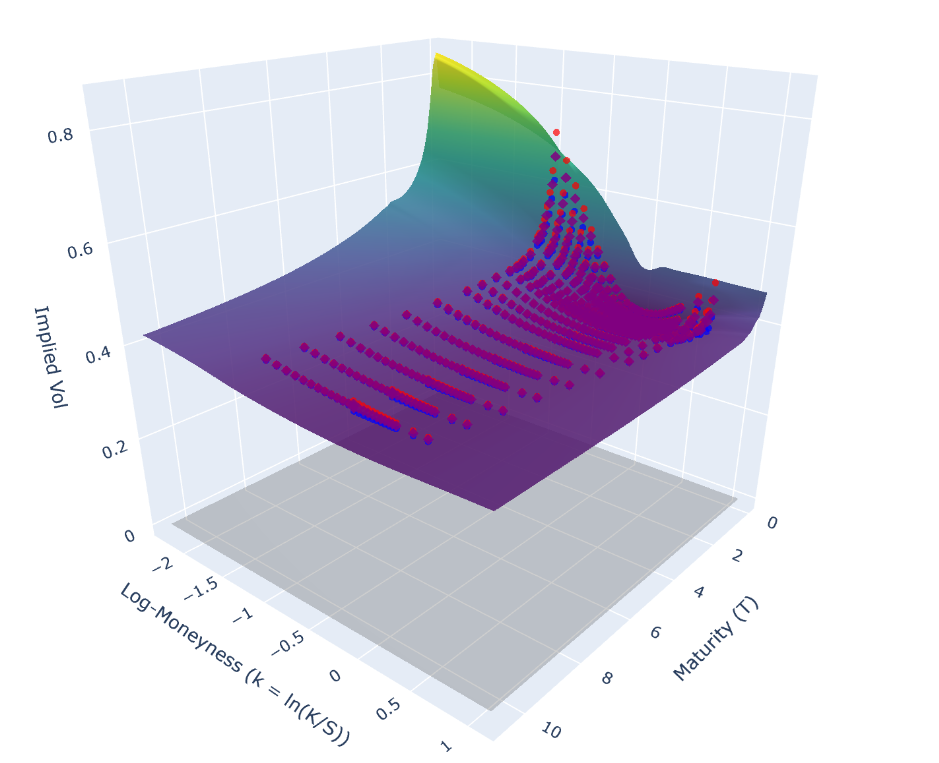
\includegraphics[width=\textwidth]{Images/surface_pinn.png}
% \caption[The L\'evy area and the lag scan]{Left}
% \label{fig:levylag}
% \end{figure}


% \begin{table}[htbp]
% \centering
% \caption{Implied Volatility Surface Calibration Summary}
% \label{tab:vol_calibration_summary}
% \begin{tabular}{lrr}
% \hline
% \textbf{Metric} & \textbf{Count} & \textbf{Percentage} \\
% \hline
% Total Quotes                 & 576 & 100.00\% \\
% Number of Smiles ($T$)       & 22  & ---      \\
% Quotes per Smile             & 26--30 & ---   \\
% Inside Bid/Ask Tunnel        & 550 & 95.49\%  \\
% Outside Bid/Ask Tunnel       & 26  & 4.51\%   \\
% \quad \textit{Below Bid}     & 11  & 1.91\%   \\
% \quad \textit{Above Ask}     & 15  & 2.60\%   \\
% \hline
% \end{tabular}
% \end{table}




\begin{figure}[H]
\centering
% --- Left Column: PINN Surface Plot ---
\begin{minipage}[t]{0.46\textwidth}
  \vspace{0pt} % Ensures top-alignment
  \centering
  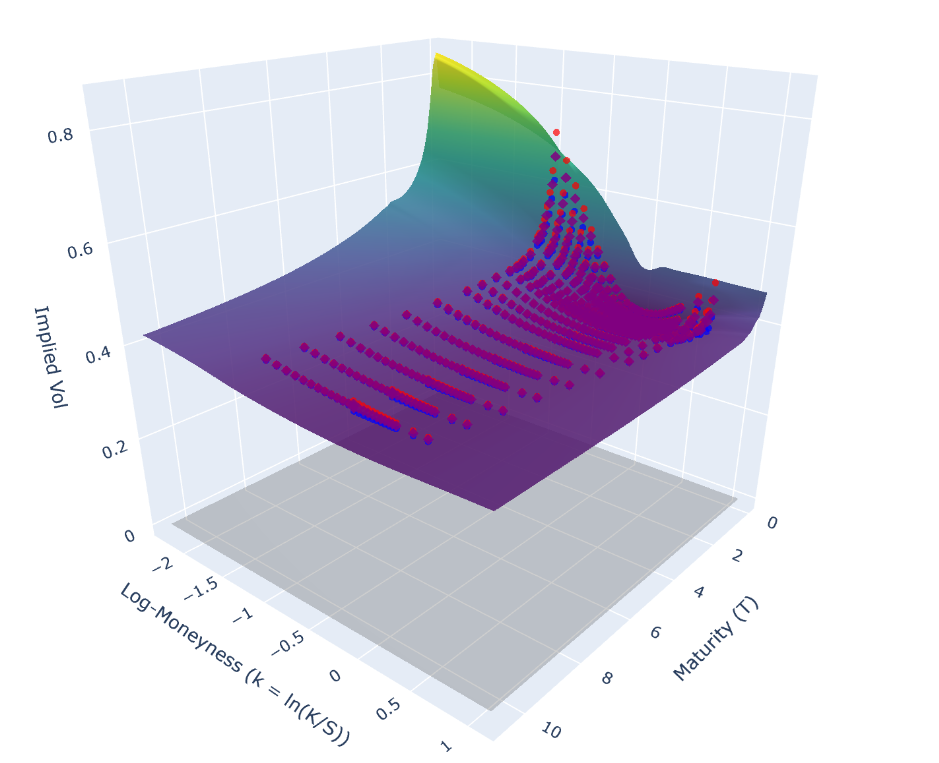
\includegraphics[width=\linewidth]{Images/surface_pinn.png}
  \caption[The fitted implied volatility surface]{Implied volatility surface representation, together with the bid (blue), ask (red) and mid (purple) quotes.}
  \label{fig:pinnsurface}
\end{minipage}\hfill
% --- Right Column: Tables ---
\begin{minipage}[t]{0.51\textwidth}
  \vspace{7pt}
  \centering
  \scriptsize % Keeps text compact to prevent column overflow
  

  
  % Table 1: Summary
  \begin{tabular}{lrr}
    \toprule
    \textbf{Metric} & \textbf{Count} & \textbf{\%} \\
    \midrule
    Total Quotes & 576 & 100.0\% \\
    Inside Bid/Ask Tunnel & 550 & 95.49\% \\
    Outside Tunnel (\textit{Below / Above}) & 26 & 4.51\% (1.9\% / 2.6\%) \\
    Smiles ($T$) & 22 & 26--30 quotes/smile \\
    \bottomrule
  \end{tabular}

  \vspace{0.8em}

  % Table 2: Breakdown
  \begin{tabular}{rrrrr}
    \toprule
    \textbf{Maturity ($T$)} & \textbf{Quotes} & \textbf{Inside} & \textbf{Outside} & \textbf{Ratio} \\
    \midrule
    0.1971 & 30 & 30 & 0 & 100.0\% \\
    0.27--0.70 (6 smiles) & 26 ea. & 26 ea. & 0 & 100.0\% \\
    0.7693 & 26 & 25 & 1 & 96.2\% \\
    1.0212 & 26 & 26 & 0 & 100.0\% \\
    1.2704 & 26 & 15 & 11 & 57.7\% \\
    1.3662 & 26 & 12 & 14 & 46.2\% \\
    1.52--9.28 (11 smiles) & 26 ea. & 26 ea. & 0 & 100.0\% \\
    \midrule
    \textbf{Total} & \textbf{576} & \textbf{550} & \textbf{26} & \textbf{95.5\%} \\
    \bottomrule
  \end{tabular}
    \captionof{table}{Calibration Summary \& Smile Breakdown.}
  \label{tab:vol_calibration_all}
\end{minipage}
\end{figure}


The tests performed, mainly for arbitrage purposes, have been passed. In terms of market fit, the main limitation has been noisy quotes as input data. Figure \ref{fig:pinnsurface} above shows the fitted surface against the quotes. It belongs to the SPX index, which is in a sense one of the most complex underlyings to calibrate due to the abundance of market data, tight bid/ask spreads and the presence of a strong skew. The errors measured to the mid are typically below five basis points, and, as Table \ref{tab:vol_calibration_all} records, $550$ of the $576$ quotes fall inside their own bid/ask, which is a good outcome given the complexity of the surface and the number of quotes fitted. The surface is smooth, and the implied volatilities are consistent with market observations. The $26$ misses are not spread across the book: $25$ of them lie on the two adjacent smiles $T=1.2704$ and $T=1.3662$, where the surface places $15$ and $12$ of $26$ quotes inside. Every other maturity is matched in full.


% \begin{table}[htbp]
% \centering
% \caption{Per-Smile Calibration Breakdown}
% \label{tab:smile_breakdown}
% \begin{tabular}{rrrrr}
% \hline
% \textbf{Maturity ($T$)} & \textbf{Quotes} & \textbf{Inside} & \textbf{Outside} & \textbf{Hit Ratio} \\
% \hline
% 0.1971 & 30 & 30 &  0 & 100.0\% \\
% 0.2738 to 0.6954 (6 smiles) & 26 each & 26 each &  0 & 100.0\% \\
% 0.7693 & 26 & 25 &  1 &  96.2\% \\
% 1.0212 & 26 & 26 &  0 & 100.0\% \\
% 1.2704 & 26 & 15 & 11 &  57.7\% \\
% 1.3662 & 26 & 12 & 14 &  46.2\% \\
% 1.5195 to 9.2813 (11 smiles) & 26 each & 26 each &  0 & 100.0\% \\
% \hline
% \textbf{Total} & \textbf{576} & \textbf{550} & \textbf{26} & \textbf{95.5\%} \\
% \hline
% \end{tabular}
% \end{table}

% ===========================================================================
\section{Calibration to Rough Heston}
\label{sec:roughcalib}

Section \ref{sec:pinn} fitted the surface with no dynamics at all: the object produced there is a
function of $(\lmon,T)$ constrained to be arbitrage-free, and nothing more. This section fits the
same quotes with the rough Heston model of Definition \ref{def:roughheston}, in which the surface is
not fitted but \emph{implied} by six numbers describing a variance process. The comparison is the
point of the chapter, and the question it answers is how much of a real index smile a two-factor
rough model can carry.

The quotes are a Totem pull for the same index and value date as \S\ref{sec:pinn}, but a
different export of it, and the objective is not that of \S\ref{subsec:objective}; the two
studies are therefore not a controlled comparison, and \S\ref{subsec:rhpinn} repeats this
calibration on the network's own book to supply one. Two
filters are applied here. Only the sixteen maturities whose $T$ is recoverable exactly are retained,
from $T=0.1040$ to $T=2.8446$; and within each of them an at-the-money cone
$|\lmon|\le\tfrac12\sqrt{T}$ is imposed, which keeps $2415$ of the $2648$ quotes. The cone is not a
convenience: its width scales as $\sqrt{T}$, so it retains a comparable range of standard deviations
at every maturity rather than a comparable range of strikes. The calibration is then performed
outright in the model parameters $(v_{0},\kappa,\theta,\xi,\rho,\Hurst)$, against the
half-spread-normalised squared error \eqref{eq:rhobjective} rather than against the composite loss
of \S\ref{subsec:objective}.


% The Hurst index $\Hurst$ is not fixed at a value
% taken from the literature but is optimised alongside $(v_{0},\kappa,\theta,\xi,\rho)$, and the
% objective is afterwards profiled in it. 

% ---------------------------------------------------------------------------
% \subsection{The quotes}
% \label{subsec:rhdata}

% The data is a single-date SPX book supplied as three sheets: a moneyness grid $\Strike/\Fwd$, a
% sheet of bid and offer implied volatilities with the corresponding mid and spread, and a sheet of
% total implied variances. Seventeen maturity columns are quoted, each with its own strike ladder of
% between $55$ and $291$ entries, padded where a maturity carries fewer strikes.

% The maturities themselves are not given as a list, and recovering them is worth one paragraph
% because the route is exact rather than fitted. Since $\tvar=\ivol^{2}T$, any column of the total
% variance sheet divided by the square of the corresponding volatility column must be constant down the
% strike ladder, and that constant is $T$. Carried out naively the quotient is not constant; carried
% out against the volatility column \emph{one place to the right} it is constant to a coefficient of
% variation of $1.2\times10^{-7}$, and the two blocks of the total variance sheet are then identified
% as $(\ivol^{\mathrm{bid}})^{2}T$ and $(\ivol^{\mathrm{ask}})^{2}T$ exactly. The total variance sheet is
% therefore displaced by one column relative to the other two. This leaves the first volatility column
% with no total variance anywhere in the file and hence no recoverable maturity; it is discarded. Its
% three signatures --- the steepest skew, the lowest at-the-money volatility and the narrowest strike
% ladder of all seventeen columns --- identify it as the shortest maturity, so what is lost is the front
% of the term structure and nothing in the interior.

% Sixteen maturities remain, from $T=0.1040$ to $T=2.8446$, carrying $2648$ quotes. Once column one is
% removed the surface is orderly: at-the-money total variance increases strictly from $0.00217$ to
% $0.09908$, so there is no calendar arbitrage in the term structure, and the $90$--$110$ skew decreases
% strictly from $0.1131$ to $0.0360$.

% Quotes are then restricted to the cone
% \begin{equation}\label{eq:cone}
%   |\lmon| \;\le\; \tfrac12\sqrt{T},
% \end{equation}
% which retains $2415$ of the $2648$. The cone is not a convenience. Its width scales as $\sqrt{T}$,
% which is the natural width of a smile, so it admits an interval of roughly constant width in the
% standardised variable $\lmon/(\ivol\sqrt{T})$: a tight collar around the money at the short end, where
% the rough model's distinctive prediction is the $T^{\Hurst-1/2}$ skew of Remark
% \ref{rem:roughhestoncost} and where the far wings are both illiquid and dominated by jump risk the
% model does not contain, and essentially the whole quoted smile at the long end. Fitting the far short-dated
% wings would spend the parameters on the part of the surface the model is least entitled to explain.

% % % ---------------------------------------------------------------------------
% \subsection{Solving the fractional Riccati}
% \label{subsec:riccatisolver}

Theorem \ref{thm:roughhestoncf} reduces pricing to \eqref{eq:fractionalriccati}, and Remark
\ref{rem:roughhestoncost} recorded the cost: the fractional derivative is non-local, so a
discretisation over $n$ steps carries the whole computed history at each step and costs $O(n^{2})$.
The solver used here is the fractional Adams predictor--corrector, vectorised across the grid
so that one solve prices an entire maturity slice. 

% \subsubsection*{The fractional integral never has to be quadratured}

The exponent of \eqref{eq:roughhestoncf} contains $I^{1-\alpha_{\Hurst}}\psi(u,\tau)$, a fractional
integral whose kernel $(\tau-s)^{-\alpha_{\Hurst}}$ is singular at the upper endpoint. Quadrature
against a singular kernel is delicate and is a standard source of order loss. It is also
unnecessary.

\begin{proposition}[Both terms of the exponent are ordinary integrals]\label{prop:noquadrature}
Let $\psi(u,\cdot)$ solve \eqref{eq:fractionalriccati} and write
$F(u,x) := \tfrac{\xi^{2}}{2}x^{2}+(\rho\xi iu-\kappa)x-\tfrac12(u^{2}+iu)$ for its right-hand side.
Then
\begin{equation}\label{eq:noquadrature}
  I^{1-\alpha_{\Hurst}}\psi(u,\tau)\;=\;\int_{0}^{\tau}F\bigl(u,\psi(u,s)\bigr)\,\dd s ,
\end{equation}
so that \eqref{eq:roughhestoncf} becomes
$\charf(u,T)=\exp\bigl(\kappa\theta\int_{0}^{T}\psi\,\dd s+v_{0}\int_{0}^{T}F(u,\psi)\,\dd s\bigr)$.
\end{proposition}

\textbf{\textit{Proof:}} The fractional derivative is
$D^{\alpha_{\Hurst}}=\frac{\dd}{\dd\tau}\circ I^{1-\alpha_{\Hurst}}$, so
\eqref{eq:fractionalriccati} states that $\frac{\dd}{\dd\tau}I^{1-\alpha_{\Hurst}}\psi=F(u,\psi)$.
Integrating from $0$ to $\tau$ and using the initial condition
$I^{1-\alpha_{\Hurst}}\psi(u,0)=0$ attached to \eqref{eq:fractionalriccati} gives
\eqref{eq:noquadrature}. \qedfilledtext

\medskip

 The predictor--corrector already evaluates $F(u,\psi)$ at every
node in order to advance, so the right-hand side of \eqref{eq:noquadrature} is available at no cost
and is integrated by the trapezoidal rule against a smooth integrand, while the left-hand side would
have required a product-integration rule against a singularity. Both terms of the exponent are then
ordinary integrals of quantities the solver has already produced.

% \subsubsection*{The pricing contour}

Prices are recovered by the Lewis form of the Fourier inversion \eqref{eq:fourierinversion},
evaluated on the line $\operatorname{Im}u=-\tfrac12$ and written for the \emph{undiscounted} call
value, so that the bond factor of \eqref{eq:fourierinversion} does not appear:
\begin{equation}\label{eq:lewis}
  \frac{C(\lmon,T)}{\Fwd}
  \;=\;1-\frac{e^{\lmon/2}}{\pi}\int_{0}^{\infty}
  \operatorname{Re}\Bigl[e^{-iu\lmon}\,\charf\bigl(u-\tfrac i2,T\bigr)\Bigr]\frac{\dd u}{u^{2}+\tfrac14}.
\end{equation}
That contour is chosen for a concrete reason: at $u\mapsto u-\tfrac i2$ the inhomogeneity of
\eqref{eq:fractionalriccati} becomes
$-\tfrac12\bigl((u-\tfrac i2)^{2}+i(u-\tfrac i2)\bigr)=-\tfrac12\bigl(u^{2}+\tfrac14\bigr)$, which is
real and negative for every $u$. The branch ambiguity that afflicts the \emph{closed-form} Heston
characteristic function does not arise here at all, \eqref{eq:fractionalriccati} being integrated
numerically; what the contour buys is a real, negative inhomogeneity, and the
$1/(u^{2}+\tfrac14)$ weight makes the tail integrable without further damping.

\subsubsection*{Where the explicit scheme breaks, and why}

The predictor--corrector is explicit and therefore has a stability limit, which is reached in
practice. Because $\psi(u,0)=0$, the first step is
approximately $\psi_{1}\approx-\tfrac12(u^{2}+\tfrac14)\,\Delta\tau^{\alpha_{\Hurst}}/\Gamma(1+\alpha_{\Hurst})$,
whereas the true solution settles near the root of the quadratic $F(u,\cdot)$, at the scale
$\bigl(\tfrac12(u^{2}+\tfrac14)\big/\tfrac{\xi^{2}}{2}\bigr)^{1/2}$. When the first step overshoots
that scale, the quadratic term dominates at the second step and the iteration diverges. Demanding no
overshoot gives the cut
\begin{equation}\label{eq:ustab}
  u_{\max}\;\le\;\frac{2\,\Gamma(1+\alpha_{\Hurst})}{\xi\,\Delta\tau^{\alpha_{\Hurst}}},
  \qquad \Delta\tau=T/n ,
\end{equation}
which is what binds at large vol-of-vol. A second, empirical, cut $u_{\max}\le c/\sqrt{T}$ with
$c=120$ binds at long maturities. Both sit far outside the region where the integrand of
\eqref{eq:lewis} is still material --- the characteristic function has decayed past $10^{-11}$ well
inside either --- so the truncation costs less than $10^{-6}$ of a vega while removing the divergence
entirely. Over a sweep of $1536$ parameter and maturity combinations spanning the whole optimisation
box, no non-finite price is produced.

% ---------------------------------------------------------------------------
\subsection{The objective}
\label{subsec:rhobjective}

Quotes are weighted by their own half-spread, so that the fit is measured in ticks rather than in
volatility points:
\begin{equation}\label{eq:rhobjective}
  \Phi(p)\;=\;\sum_{i}\left(\frac{\ivol^{p}(\lmon_{i},T_{i})-\ivol^{\mathrm{mid}}(\lmon_{i},T_{i})}
  {h_{i}}\right)^{2},
  \qquad h_{i}=\tfrac12\bigl(\ivol^{\mathrm{ask}}-\ivol^{\mathrm{bid}}\bigr)(\lmon_{i},T_{i}),
\end{equation}
the sum running over the quotes.

The parameter vector is $p=(v_{0},\kappa,\theta,\xi,\rho,\Hurst)$, all six free, searched by
differential evolution over the box of Table \ref{tab:rhbounds} and then polished by Nelder--Mead at a
finer time grid. No parameter is fixed and no penalty or prior is imposed, so the fit reported below
is what the surface alone asks for.

\begin{table}[H]
\centering
\small
\begin{tabular}{llp{7.6cm}}
\hline
Parameter & Box & Reading\\
\hline
$v_{0}$ & $[0.0025,\,0.16]$ & Spot variance; the box is volatility between $5\%$ and $40\%$.\\
$\theta$ & $[0.0025,\,0.16]$ & Long variance, same box.\\
$\kappa$ & $[0.05,\,10]$ & Mean reversion. In a rough model this is weakly identified: the kernel
  already supplies the decay of the term structure.\\
$\xi$ & $[0.05,\,1.5]$ & Vol-of-vol; also the parameter that drives the stability cut
  \eqref{eq:ustab}.\\
$\rho$ & $[-0.999,\,-0.05]$ & Spot/vol correlation, constrained negative: the sign of the equity skew
  is not in question.\\
$\Hurst$ & $[0.02,\,0.50]$ & Hurst index. The upper endpoint is the classical Heston case, so the
  box \emph{contains} the non-rough model and does not assume the conclusion.\\
\hline
\end{tabular}
\caption[The optimisation box]{The optimisation box. Only $\rho$ is sign-constrained; the Hurst index is free over the
whole admissible range, including its classical endpoint.}
\label{tab:rhbounds}
\end{table}

% ---------------------------------------------------------------------------
% \subsection{Validating the pricer}
% \label{subsec:rhvalidation}

% A calibration reports a number whether or not the pricer beneath it is correct, so the pricer is
% tested first, against cases with known answers. Three tests are used and all are passed before any
% fitting is attempted.

% \begin{itemize}
%   \item \textbf{The degenerate case.} Setting $\xi=0$ and $v_{0}=\theta$ freezes the variance at
%     $v_{0}$ for \emph{every} $\Hurst$, since the convolution in \eqref{eq:roughheston} then acts on a
%     constant. The model is Black--Scholes and the implied volatility must equal $\sqrt{v_{0}}$ at
%     every strike and maturity. It does, to $1.5\times10^{-6}$, for $\Hurst\in\{0.05,0.12,0.35,0.5\}$.
%     This is an end-to-end test: it exercises the Riccati solve, the contour integral
%     \eqref{eq:lewis} and the volatility inversion together, and it is sensitive to an error in any of
%     them.
%   \item \textbf{The classical endpoint.} At $\Hurst=\tfrac12$ the fractional derivative is an
%     ordinary one and \eqref{eq:fractionalriccati} is a Riccati ODE. Solved independently to a
%     tolerance of $10^{-11}$, the reference agrees with the Adams scheme with errors
%     $5.2\times10^{-4}$, $1.3\times10^{-4}$, $3.2\times10^{-5}$, $7.9\times10^{-6}$ at
%     $n=100,200,400,800$: a ratio of $4$ per doubling, which is the second-order convergence the
%     scheme is supposed to have.
%   \item \textbf{Deterministic but non-constant variance.} Setting $\xi=0$ with $v_{0}\neq\theta$ and
%     $\alpha_{\Hurst}=1$ leaves $v_{t}=\theta+(v_{0}-\theta)e^{-\kappa t}$, so the implied volatility
%     must be $\bigl(\theta+(v_{0}-\theta)(1-e^{-\kappa T})/(\kappa T)\bigr)^{1/2}$ exactly. Over a
%     range of $(v_{0},\theta,\kappa)$ and maturities this holds to about $10^{-7}$. Unlike the previous
%     test this one is sensitive to $\kappa$ and $\theta$ separately, and it is the check that
%     the two terms of \eqref{eq:noquadrature} are combined with the right coefficients.
%   \item \textbf{The roughness itself.} The tests above would all pass for a solver that ignored
%     $\Hurst$. This one does not: fitting the model's own short-dated at-the-money skew to a power of
%     $T$ returns exponents $-0.494,-0.450,-0.342,-0.222,-0.103,+0.008$ at
%     $\Hurst=0.05,0.10,0.20,0.30,0.40,0.50$, against the predicted $\Hurst-\tfrac12$ of
%     $-0.45,-0.40,-0.30,-0.20,-0.10,0$. The scheme therefore reproduces the skew power law of Remark
%     \ref{rem:roughhestoncost}, including its collapse to a flat skew at the classical endpoint.
%   \item \textbf{Grid convergence and robustness.} Against a reference at $n=1600$, prices at $n=300$
%     are accurate to about $10^{-6}$, which is some $10^{-5}$ in volatility, two orders inside the
%     median half-spread. The sweep over $1536$ parameter and maturity combinations mentioned above
%     returns no non-finite value.
% \end{itemize}

% The volatility inversion is a safeguarded Newton iteration run on the whole surface at once, started
% from the market volatility and falling back to bisection where vega collapses; it reproduces a
% scalar Brent inversion to $2.5\times10^{-11}$ while being some two orders of magnitude faster, which
% matters only because \eqref{eq:rhobjective} is evaluated a few thousand times.


% ---------------------------------------------------------------------------
\subsection{Results}
\label{subsec:rhresults}

Table \ref{tab:rhfit} reports the fit. The global search was a differential evolution over the box of
Table \ref{tab:rhbounds} on a coarse time grid, followed by a bounded local polish on a fine one.
The polish is bounded by the same box, which is why $\Hurst$ reaches its endpoint and does not pass it.

\begin{table}[H]
\centering
\small
\begin{tabular}{lrl}
\hline
Parameter & Value & \\
\hline
$v_{0}$ & $0.02368$ & spot volatility $\sqrt{v_{0}}=15.39\%$\\
$\theta$ & $0.06247$ & long volatility $\sqrt{\theta}=24.99\%$\\
$\kappa$ & $2.1184$ & \\
$\xi$ & $0.9220$ & \\
$\rho$ & $-0.7347$ & \\
$\Hurst$ & $0.5000$ & \emph{at the smooth end} of the box $[0.02,\,0.50]$; $\alpha_{\Hurst}=1.00$\\
\hline
$\Phi$ & $76\,160$ & $\Phi/n=31.54$ on $n=2415$ quotes\\
RMSE & $43.6$ bp & of volatility\\
inside bid/ask & $10.3\%$ & median half-spread $5.5$ bp\\
\hline
\end{tabular}
\caption[Rough Heston calibrated to the SPX book]{Rough Heston calibrated to $2415$ SPX quotes, all six
parameters free. The Hurst index lands on the upper endpoint of its admissible range,
at which $\alpha_{\Hurst}=1$ and \eqref{eq:roughheston} \emph{is} the classical Heston system
\eqref{eq:heston}. A control fitted on the same sample with $\Hurst$ pinned at $\tfrac12$
reproduces every entry of this table, and its objective agrees with the one above to nine
significant figures.}
\label{tab:rhfit}
\end{table}

One parameter check is worth recording. Here $2\kappa\theta = 0.265$ against $\xi^{2}=0.850$, so the
Feller condition \eqref{eq:fellercondition} fails; and since $\Hurst=\tfrac12$ the variance is
exactly the square-root process of Example \ref{example:cirwellposed}, so Proposition
\ref{prop:feller} applies verbatim and the calibrated variance reaches the origin with positive
probability. This is the behaviour Subsection \ref{subsec:stochvol} anticipated, and it is the price
of a steep short-dated skew.



% The bottom row of Figure \ref{fig:rhsmiles} shows something else worth recording: at $T=0.104$ the
% residual oscillates by tens of half-spreads from strike to adjacent strike. A misspecified model
% produces smooth residuals, not jagged ones, so part of what the objective is being asked to fit at the
% short end is quote noise in excess of the quoted spread. The shortest maturity is simultaneously the
% most heavily weighted and the least internally consistent.

\begin{figure}[H]
\centering
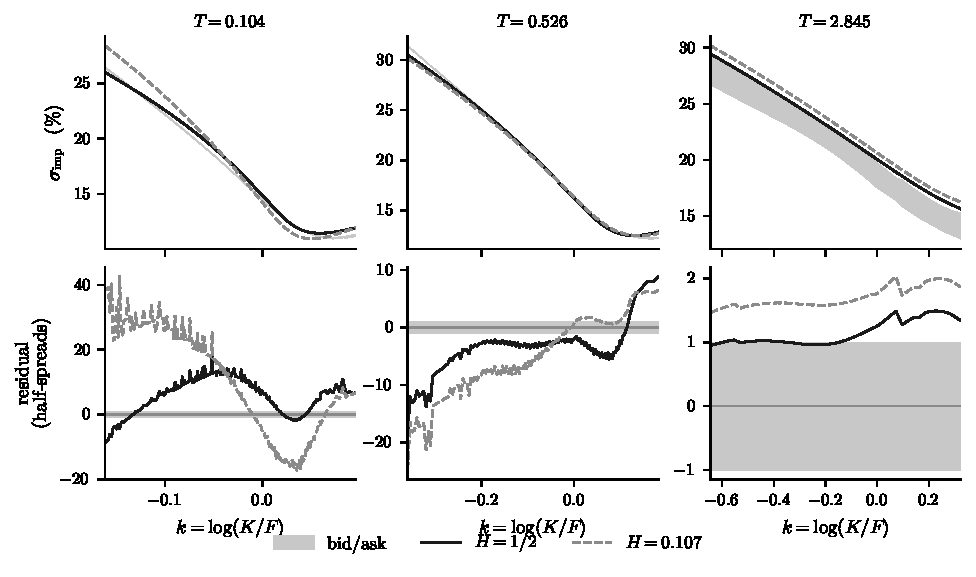
\includegraphics[width=\textwidth]{Images/rh-smiles.pdf}
\caption[Rough Heston fit by maturity]{The calibrated model against the market at three maturities. Top: implied volatility, with the bid/ask band shaded. Bottom: the
residual in half-spread units, the shaded strip being $\pm1$ half-spread. The two rows disagree about
where the model fails, and the disagreement is entirely the term structure of the spread: at
$T=2.845$ the model is more than a volatility point away and still inside two half-spreads, while at
$T=0.104$ it is a quarter of that distance away and tens of half-spreads out.}
\label{fig:rhsmiles}
\end{figure}

\begin{table}[H]
\centering
\small
\begin{tabular}{rrrrrrr}
\hline
$T$ & quotes & med.\ $h$ (bp) & RMSE (bp) & bias (bp) & \% of $\Phi$ & \% of $\Hurst$ gap\\
\hline
$0.1040$ & $256$ & $5.6$ & $46.6$ & $+35.7$ & $\mathbf{24.1}$ & $\mathbf{+56.9}$\\
$0.1807$ & $266$ & $5.8$ & $29.7$ & $+0.7$ & $9.3$ & $+9.1$\\
$0.2574$ & $212$ & $4.8$ & $31.1$ & $-9.5$ & $15.5$ & $+0.0$\\
$0.3504$ & $210$ & $4.7$ & $22.0$ & $-8.3$ & $4.8$ & $-1.7$\\
$0.4298$ & $118$ & $4.5$ & $28.1$ & $-20.7$ & $5.6$ & $-0.3$\\
$0.5257$ & $126$ & $4.2$ & $28.4$ & $-17.9$ & $4.9$ & $+4.2$\\
$0.6023$ & $132$ & $4.4$ & $29.5$ & $-17.4$ & $3.9$ & $+5.8$\\
$0.6790$ & $134$ & $4.9$ & $23.1$ & $-16.1$ & $3.2$ & $+6.7$\\
$0.7748$ & $146$ & $4.9$ & $27.0$ & $-8.7$ & $4.6$ & $+9.6$\\
$0.8515$ & $147$ & $5.8$ & $23.6$ & $+8.2$ & $2.8$ & $+4.4$\\
$0.9281$ & $147$ & $6.6$ & $29.5$ & $+21.0$ & $4.3$ & $+2.9$\\
$1.0240$ & $145$ & $7.5$ & $36.0$ & $+22.6$ & $5.1$ & $+2.8$\\
$1.1006$ & $160$ & $8.3$ & $43.6$ & $+42.7$ & $5.8$ & $-0.3$\\
$1.3470$ & $\;\;99$ & $10.8$ & $76.7$ & $+71.6$ & $5.1$ & $-0.2$\\
$1.8480$ & $\;\;62$ & $29.1$ & $110.6$ & $+104.4$ & $1.0$ & $+0.2$\\
$2.8446$ & $\;\;55$ & $109.9$ & $131.7$ & $+130.0$ & $0.1$ & $+0.1$\\
\hline
\end{tabular}
\caption[Fit by maturity]{Fit by maturity at the parameters of Table \ref{tab:rhfit}. The last two columns are the
share of the objective $\Phi$ contributed by each maturity, and that maturity's share of the gap
$\Phi(\Hurst{=}0.107)-\Phi(\Hurst{=}\tfrac12)$. In volatility the error grows with maturity; weighted by
the spread the order reverses, and the shortest maturity carries both a quarter of the objective and
well over half of the preference for the smooth kernel.}
\label{tab:rhpermat}
\end{table}

Three things must be said about this table before anything is concluded from it.

\emph{The fit is mediocre in absolute terms.} A root mean square error of $44$ basis points against a
median half-spread of $5.5$ is eight half-spreads, and only $10.3\%$ of quotes are matched inside their
own bid/ask. Six parameters do not span sixteen maturities of SPX. Figure \ref{fig:rhsmiles} shows
the shape of the failure and Table \ref{tab:rhpermat} localises it.

\emph{Where the failure sits depends on the units.} Measured in
volatility the error grows with maturity: about $25$ basis points from three months to one year,
rising monotonically to a \emph{bias} of $+130$ at $T=2.84$, where bias and RMSE are $130.0$ and
$131.7$ so that essentially the whole error is a parallel offset. Measured in half-spreads --- which
is the metric \eqref{eq:rhobjective} actually minimises --- the ranking reverses completely, because
the market quotes the long end $20$ times more loosely than the short one: the median half-spread runs
from $4.5$ basis points around six months to $109.9$ at the longest maturity. 

\emph{The Hurst index goes to the smooth boundary.} This is the opposite of what Chapter
\ref{ch:roughpaths} would lead one to expect, and it is not a numerical accident. Table
\ref{tab:rhprofile} profiles the objective in $\Hurst$, re-optimising the other five parameters at
each fixed value.

\begin{table}[H]
\centering
\small
\begin{tabular}{rrrrrrr}
\hline
$\Hurst$ & $\Phi/n$ & $v_{0}$ & $\theta$ & $\kappa$ & $\xi$ & $\rho$\\
\hline
$0.030$ & $115.65$ & $0.0223$ & $0.1599^{*}$ & $0.253$ & $0.359$ & $-0.710$\\
$0.068$ & $\;98.17$ & $0.0228$ & $0.1600^{*}$ & $0.260$ & $0.377$ & $-0.715$\\
$0.107$ & $\;82.83$ & $0.0231$ & $0.1600^{*}$ & $0.267$ & $0.392$ & $-0.721$\\
$0.145$ & $\;69.62$ & $0.0233$ & $0.1600^{*}$ & $0.276$ & $0.413$ & $-0.724$\\
$0.183$ & $\;58.65$ & $0.0236$ & $0.1600^{*}$ & $0.286$ & $0.434$ & $-0.726$\\
$0.222$ & $\;50.10$ & $0.0238$ & $0.1600^{*}$ & $0.297$ & $0.458$ & $-0.727$\\
$0.260$ & $\;44.21$ & $0.0240$ & $0.1599^{*}$ & $0.309$ & $0.484$ & $-0.728$\\
$0.298$ & $\;41.00$ & $0.0241$ & $0.1391$ & $0.391$ & $0.521$ & $-0.730$\\
$0.337$ & $\;38.62$ & $0.0240$ & $0.1032$ & $0.637$ & $0.582$ & $-0.731$\\
$0.375$ & $\;36.49$ & $0.0239$ & $0.0857$ & $0.917$ & $0.649$ & $-0.732$\\
$0.413$ & $\;34.61$ & $0.0239$ & $0.0753$ & $1.235$ & $0.724$ & $-0.733$\\
$0.452$ & $\;33.03$ & $0.0238$ & $0.0684$ & $1.596$ & $0.806$ & $-0.734$\\
$0.490$ & $\;31.79$ & $0.0237$ & $0.0635$ & $2.003$ & $0.897$ & $-0.735$\\
$0.500$ & $\;\mathbf{31.54}$ & $0.0237$ & $0.0625$ & $2.118$ & $0.922$ & $-0.735$\\
\hline
\end{tabular}
\caption[The objective profiled in the Hurst index]{The objective profiled in $\Hurst$. Entries marked $^{*}$ sit on the upper bound of
$\theta$. The profile decreases strictly at every step of the grid: every rougher kernel on it
fits worse.}
\label{tab:rhprofile}
\end{table}

The profile decreases strictly at every step of the grid. At $\Hurst=0.107$, a value typical of the
rough volatility literature, the objective is $2.6$ times its value at the endpoint. Four checks
were made before reading anything into this.

\begin{itemize}
  \item \textbf{Is it the box?} For $\Hurst\le0.26$ the fitted $\theta$ sits on its upper bound, so
    those rows are constrained. Re-optimising with $\theta$ allowed up to $0.80$ --- a long-run
    volatility of $89\%$, economically absurd --- improves $\Hurst=0.107$ only from $\Phi/n=82.8$ to
    $70.3$, and does so by driving $\kappa$ to $0.042$. Meanwhile the same widening leaves $\Phi/n$
    and $\theta$ at $\Hurst=0.490$ and $\Hurst=0.375$ unchanged to four decimal places: those
    optima are interior. Even granted absurd parameters the rough kernel fits more than twice as badly
    as the smooth one does at its own interior optimum.
  \item \textbf{Is it the search?} No. A global search and an independent local restart from a
    different starting point return the same endpoint, agreeing in $\Phi$ to ten significant
    figures.
  \item \textbf{Is it the solver?} No. Fitting the model's \emph{own} short-dated at-the-money skew
    to a power of $T$ returns an exponent close to the predicted $\Hurst-\tfrac12$ throughout the
    range: $-0.494$ against $-0.45$ at $\Hurst=0.05$, $-0.342$ against $-0.30$ at $\Hurst=0.20$,
    and $+0.008$ against $0$ at the classical endpoint. The roughness is present in the prices the
    solver produces.
  \item \textbf{Is it the forward convention?} No. If the supplied moneyness were $\Strike/\Spot$
    rather than $\Strike/\Fwd$ the model would inherit a maturity-proportional strike offset, which is
    exactly the shape of the long-dated bias in Table \ref{tab:rhpermat}. It is not: the smile minimum
    sits at $1.7$ to $2.1$ standard deviations $\ivol\sqrt{T}$ above the money at every one of the
    sixteen maturities, with no trend. A spot convention would make that ratio grow like $\sqrt{T}$.
\end{itemize}

% % ---------------------------------------------------------------------------
\subsection{What the surface can and cannot identify}
\label{subsec:rhidentification}

It would be easy, and wrong, to report Table \ref{tab:rhprofile} as evidence that this index is not
rough without first asking whether the fit can see $\Hurst$ at all. Two estimators are in play and
they must be kept apart: the at-the-money skew regression, which is what the rough volatility
literature reads $\Hurst$ off, and the objective \eqref{eq:rhobjective} itself. The first has no
power over this maturity range, as the rest of this subsection shows. The second does, and
\S\ref{subsec:rhplant} shows it by planting a known $\Hurst$ and recovering it. The distinction is
the whole of the matter: an inference from the blindness of the one to the blindness of the other is
exactly the step that does not hold.

The argument rests on one measurement. Remark \ref{rem:roughhestoncost} identified the empirical
signature of roughness as the at-the-money skew power law $T^{\Hurst-1/2}$, and it is natural to
estimate $\Hurst$ by regressing the log skew on the log maturity. Doing so on the market quotes gives
a slope of $-0.454$, that is $\Hurst\approx0.046$: a strongly rough reading, apparently in flat
contradiction with Table \ref{tab:rhprofile}. The contradiction dissolves when the same estimator is
applied to the fitted models themselves.

\begin{table}[H]
\centering
\small
\begin{tabular}{lrr}
\hline
Skew regressed over $T\in[0.104,\,2.845]$ & slope & implied $\Hurst$\\
\hline
market quotes & $-0.454$ & $0.046$\\
model at $\Hurst=\tfrac12$ & $-0.475$ & $0.025$\\
model at $\Hurst=0.107$ & $-0.506$ & $-0.006$\\
\hline
\end{tabular}
\caption[The skew power law over the available range]{The skew power law estimated over the available maturity range, applied to the market and to
two calibrated models whose true Hurst indices differ by a factor of nearly five. The estimator
cannot tell them apart. The legend of Figure \ref{fig:rhidentification} reports the same three
slopes.}
\label{tab:rhskewexponent}
\end{table}

\begin{figure}[H]
\centering
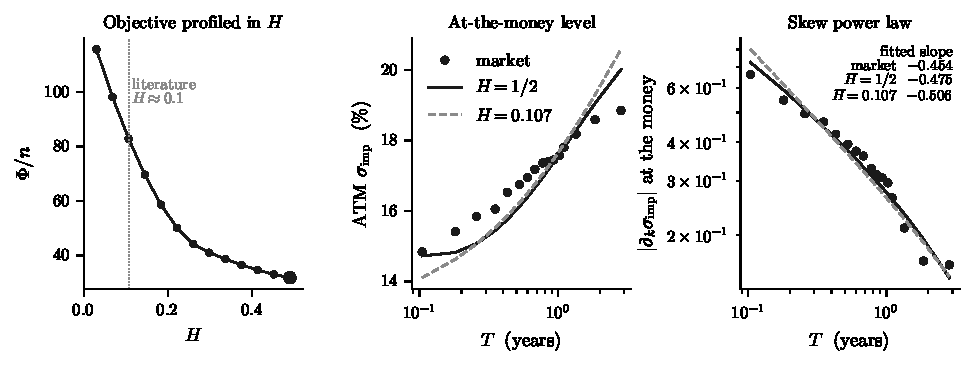
\includegraphics[width=\textwidth]{Images/rh-identification.pdf}
\caption[What the surface identifies]{Left: the objective profiled in $\Hurst$, the other five
parameters re-optimised at each point; it decreases at every step and its least value on the
grid drawn is $\Hurst=\tfrac12$, marked. Centre: the at-the-money term structure, market against the two calibrated
models. Right: the same two models and the market on log axes, with the fitted slopes of
$|\partial_{\lmon}\ivol|$ against $T$. The three slopes agree to within $0.06$ although the two models
differ in $\Hurst$ by a factor of nearly five, which is Table \ref{tab:rhskewexponent} drawn: over
this maturity range the skew power law does not separate rough from smooth.}
\label{fig:rhidentification}
\end{figure}

The model at $\Hurst=\tfrac12$ --- the classical endpoint itself --- reproduces the
``rough'' exponent $-0.475$ essentially as well as the genuinely rough model reproduces $-0.506$, and
both lie on the same side of the market's $-0.454$, within $0.06$ of it. The estimator has no power here, and the reason is that
$T^{\Hurst-1/2}$ is an asymptotic statement as $T\to0$. Over a range beginning at $38$ days, the
mean reversion of \emph{any} Heston-type model decays the skew on its own, and that decay dominates
the contribution of the kernel.

One entry of Table \ref{tab:rhskewexponent} deserves a line of its own. The implied $\Hurst$ read
off the rough model is $-0.006$, outside the admissible range $(0,\tfrac12)$ altogether. That is not
a property of the model, whose $\Hurst$ is $0.107$ by construction, but of the estimator: over this
maturity range the regression does not recover the exponent it is meant to measure, and nothing
constrains the value it returns to be admissible. An estimate that lands outside the parameter space
is the clearest possible symptom of the identification failure this subsection is about.

% ---------------------------------------------------------------------------
\subsection{Planting a known Hurst index}
\label{subsec:rhplant}

Table \ref{tab:rhprofile} and Table \ref{tab:rhskewexponent} are both read off the market, where the
answer is unknown. The question they raise --- whether the objective can identify $\Hurst$ on a grid
of this shape --- can be settled on a book whose answer is known, because we build it.

Take the sixteen maturities, the strike ladder and the cone of the real sample; price them with
\eqref{eq:roughheston} at the parameters of Table \ref{tab:rhfit} but with $\Hurst=0.10$; and
perturb each quote by a Gaussian draw of one standard half-spread. The result carries the geometry
and the noise of the market and a Hurst index of exactly $0.10$. Since
$\E[(\text{noise}/h)^{2}]=1$ by construction, the objective at the planted parameters must be
$\Phi/n=1$; it is $1.003$, which is the first check that the book is what it claims to be.

\begin{table}[H]
\centering
\small
\begin{tabular}{lrrrrr}
\hline
 & $v_{0}$ & $\theta$ & $\kappa$ & $\xi$ & $\rho$\\
\hline
planted & $0.023679$ & $0.062474$ & $2.11842$ & $0.92200$ & $-0.73474$\\
recovered at $\Hurst=0.10$ & $0.023670$ & $0.062400$ & $2.12494$ & $0.92256$ & $-0.73481$\\
\hline
\end{tabular}
\caption[Planted and recovered parameters]{The five nuisance parameters planted in the synthetic book and those returned by the
calibration with $\Hurst$ held at the planted value. The search is the one behind Table
\ref{tab:rhfit}: differential evolution followed by a bounded polish.}
\label{tab:rhplant}
\end{table}

Run at $\Hurst=0.10$ the calibration returns $\Phi/n=1.001$ --- the noise floor --- and the five
parameters of Table \ref{tab:rhplant}. Run at $\Hurst=\tfrac12$ on the same book it returns $55.3$.
Set that beside the market book and the contrast is the point:

\begin{table}[H]
\centering
\small
\begin{tabular}{lrr}
\hline
$\Phi/n$ at & $\Hurst\approx0.1$ & $\Hurst=\tfrac12$\\
\hline
the synthetic book, planted rough & $\mathbf{1.00}$ & $55.3$\\
the market book of Table \ref{tab:rhfit} & $82.7$ & $\mathbf{31.5}$\\
\hline
\end{tabular}
\caption[Rough and smooth kernels on both books]{The objective on a book that is rough by construction and on the market book, at the two
ends of the admissible range. On the first the rough kernel wins by a factor of fifty; on the second
the smooth kernel wins by a factor of $2.6$. Every entry is a global search, so the four are
like for like: the market entry at $\Hurst\approx0.1$ is a fit at $\Hurst=0.107$ returning $82.71$
against the $82.83$ of Table \ref{tab:rhprofile}, and the synthetic entry at $\Hurst=\tfrac12$
returns $55.30$. There the smooth kernel drives $\xi$ to its upper bound trying to carry a roughness
it does not have, which is the mirror of what $\theta$ does on the market book at small $\Hurst$.}
\label{tab:rhplantcompare}
\end{table}

The objective therefore separates a rough book from a smooth one by a wide margin, on exactly the
grid the market book occupies and at exactly its noise level. Table \ref{tab:rhskewexponent} shows
that the skew regression cannot tell the two apart; this shows that the calibration can. What the
market book says is accordingly not that $\Hurst$ is unknowable here, but that this surface is not
rough within this model family --- and the reason the profile slides to the endpoint is the one
\S\ref{subsec:rhpinn} reads off the quotes directly, a term structure of the at-the-money level that
no one-factor Heston can thread at any $\Hurst$.

One caveat remains, and it concerns the instrument rather than the conclusion. The profile of Table
\ref{tab:rhprofile} re-optimises the five nuisance parameters by a Nelder--Mead continuation,
walking $\Hurst$ down from the smooth end. On the synthetic book that procedure reports
$\Phi/n=19.6$ at $\Hurst=0.124$, where $1.003$ is attainable: carried down from $\tfrac12$ it never
reaches the basin a rough kernel needs. A profile built that way is an \emph{upper bound} on
$\Phi^{*}(\Hurst)$. On the market book the bound is tight --- the independent global search quoted
above agrees with it to $0.14\%$, and on the same five parameters --- because there is no distant
rough basin to miss. On a book that has one, there is, and a profile alone would not have found it.

% ---------------------------------------------------------------------------
\subsection{The same book as \S\ref{sec:pinn}}
\label{subsec:rhpinn}

One thing has been left implicit. The sample fitted above is not the one \S\ref{sec:pinn} trained on.
Both are Totem consensus pulls for the same index and the same value date, but they are different
exports: the network was given $576$ quotes on $22$ maturities reaching $T=9.28$, while
\eqref{eq:rhobjective} was minimised over the $2415$ quotes of a denser sixteen-maturity grid that
stops at $T=2.84$. Nothing said so far depends on the difference, but a comparison between the two
methods does, so the calibration is repeated here on the network's own book.

Two filters are applied, and to the rough Heston fit alone: maturities out to one year, which leaves
the eight shortest smiles, and an at-the-money cone $|\lmon|\le\tfrac12\sqrt{T+0.1}$, which keeps
$133$ of the $212$ quotes in that range. The network was fitted to the whole book.

\begin{table}[H]
\centering
\small
\begin{tabular}{lrl}
\hline
Parameter & Value & \\
\hline
$v_{0}$ & $0.14412$ & spot volatility $\sqrt{v_{0}}=37.96\%$\\
$\theta$ & $0.13592$ & long volatility $\sqrt{\theta}=36.87\%$\\
$\kappa$ & $6.6187$ & \\
$\xi$ & $1.2578$ & \\
$\rho$ & $-0.1234$ & \\
$\Hurst$ & $0.500000$ & \emph{at the smooth end} of the box $[0.02,\,0.50]$\\
\hline
$\Phi$ & $2588.5$ & $\Phi/n=19.46$ on $n=133$ quotes\\
RMSE & $58.4$ bp & of volatility; largest error $160.7$ bp\\
inside bid/ask & $20.3\%$ & median half-spread $11.1$ bp\\
\hline
\end{tabular}
\caption[Rough Heston on the network's own book]{Rough Heston calibrated to the $133$ quotes of the book of \S\ref{sec:pinn} with $T\le1$
lying inside the cone $|\lmon|\le\tfrac12\sqrt{T+0.1}$, all six parameters free. As in Table
\ref{tab:rhfit} the Hurst index goes to the upper endpoint of its range; a control with $\Hurst$
pinned at $\tfrac12$ reproduces every entry above to six decimal places.}
\label{tab:rhpinn}
\end{table}

The free search returns $\Hurst=0.500000$. Pinning $\Hurst$ at $\tfrac12$ and refitting the other
five parameters reproduces every entry of the table to six decimal places, and the profile falls
strictly from $\Phi/n=21.15$ at $\Hurst=0.05$ to $19.46$ at the endpoint. A second book, on a
different maturity grid, therefore returns the answer the first one did: left free, the calibration
selects its own classical limit.

Here $2\kappa\theta = 1.799$ against $\xi^{2}=1.582$, so this fit satisfies the Feller condition
\eqref{eq:fellercondition} that the one of Table \ref{tab:rhfit} violates.

The absolute fit is worse than in Table \ref{tab:rhfit} --- $58$ basis points against a median
half-spread of $11$ --- and the reason has nothing to do with the kernel. It is in the third column
of Table \ref{tab:rhpinnmat}.

\begin{table}[H]
\centering
\small
\begin{tabular}{rrrrrrr}
\hline
$T$ & quotes & ATM $\ivol$ & med.\ $h$ (bp) & RMSE (bp) & bias (bp) & inside\\
\hline
$0.1971$ & $16$ & $0.3692$ & $14.5$ & $78.4$ & $-76.5$ & $0.0\%$\\
$0.2738$ & $14$ & $0.3554$ & $18.9$ & $57.7$ & $+53.9$ & $0.0\%$\\
$0.3504$ & $15$ & $0.3476$ & $15.0$ & $123.6$ & $+122.5$ & $0.0\%$\\
$0.4463$ & $16$ & $0.3627$ & $10.9$ & $34.2$ & $-30.8$ & $12.5\%$\\
$0.5229$ & $18$ & $0.3577$ & $\;\;8.9$ & $15.9$ & $-1.9$ & $61.1\%$\\
$0.5996$ & $18$ & $0.3531$ & $\;\;9.4$ & $46.3$ & $+44.7$ & $5.6\%$\\
$0.6954$ & $18$ & $0.3580$ & $10.3$ & $12.5$ & $-4.3$ & $50.0\%$\\
$0.7693$ & $18$ & $0.3602$ & $\;\;8.1$ & $28.0$ & $-24.6$ & $22.2\%$\\
\hline
\end{tabular}
\caption[Fit by maturity on the network's book]{The fit of Table \ref{tab:rhpinn} by maturity. The third column is the market
at-the-money volatility, taken from the quote nearest $\lmon=0$; it changes direction three times.
A Heston at-the-money term structure cannot, at any $\Hurst$.}
\label{tab:rhpinnmat}
\end{table}

The at-the-money level does not fall monotonically. It descends to $0.3476$ at $T=0.35$, recovers to
$0.3627$ at $T=0.45$, dips again and rises again: three changes of direction across eight maturities.
A one-factor Heston term structure interpolates between $\sqrt{v_{0}}$ and $\sqrt{\theta}$ at the
single rate $\kappa$, and is therefore monotone in $T$ for every admissible parameter set, $\Hurst$
included. It cannot thread that shape, and the bias column records the consequence: it alternates in
sign --- $-76$, $+54$, $+123$, $-31$, $-2$, $+45$, $-4$, $-25$ basis points --- rather than drifting
one way, as a misspecified kernel would make it. The two maturities the model does reach, $T=0.52$
and $T=0.70$, are the two that happen to sit on a monotone path through the rest.

The optimiser pays for the attempt in the parameters. It drives $\xi$ to $1.26$ and puts both
$v_{0}$ and $\theta$ in the upper part of their boxes, and it returns $\rho=-0.12$: an implausibly
weak spot/volatility correlation for an equity index, and the signature of a fit spending its skew on
a level mismatch it cannot repair.

Figure \ref{fig:rhpinncompare} places both methods on the two smiles the diffusion fits best. Where
it attains root mean square errors of $15.9$ and $12.5$ basis points, the network attains $3.2$ and
$4.2$, against half-spreads of $8.9$ and $10.3$: it is inside the quoted band at every strike of
both, and its residual is of the order of a third of a half-spread rather than two.

\begin{figure}[H]
\centering
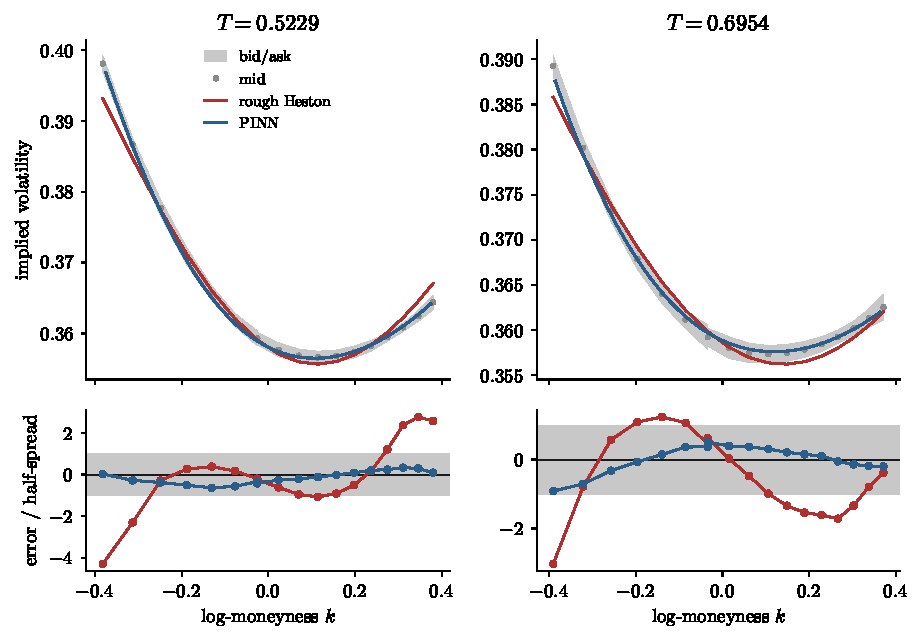
\includegraphics[width=\textwidth]{Images/pinn-heston-compare.pdf}
\caption[Heston and the network on two smiles]{The two maturities of Table
\ref{tab:rhpinnmat} at which the diffusion comes closest to the quoted spread, with the surface of
\S\ref{sec:pinn} drawn alongside it. Top: implied volatility, the bid/ask band shaded. Bottom: the
error in half-spread units, the shaded strip being $\pm1$ half-spread. Across the $36$ strikes shown
the network stays inside the band at every one and the diffusion at $20$.}
\label{fig:rhpinncompare}
\end{figure}

Two conclusions follow, and they are of different kinds. The first concerns the model: on this book,
as on the other, nothing is gained by letting $\Hurst$ leave $\tfrac12$, and what defeats the fit is
the term structure of the at-the-money level rather than the roughness of the kernel. That is the
diagnosis \S\ref{subsec:rhidentification} reached by reading the profile; here it is reached from the
quotes themselves, which is the stronger route to it.

The second concerns the comparison, and it should be stated without decoration. The network places
$550$ of $576$ quotes inside their own bid/ask across $22$ maturities; the diffusion places $27$ of
$133$ inside across eight. This is not a contest between two theories of volatility and is not
offered as one --- the objectives differ, and \S\ref{subsec:objective} fits a surface where
\eqref{eq:rhobjective} fits a dynamic model. It is the price of a parametrisation, and the price is
large: what the six parameters buy is an arbitrage-free model of the spot with an interpretable
$\rho$, a $\kappa$ and a $\theta$, and what they cost is every basis point of the gap above.

% Two consequences follow.

% First, the preference recorded in Table \ref{tab:rhprofile} is decided almost entirely at the short
% end. The last column of Table \ref{tab:rhpermat} attributes $57.3\%$ of the gap between
% $\Hurst=0.107$ and $\Hurst=0.49$ to the single maturity $T=0.1040$, and $67.2\%$ to the first three;
% the two longest maturities together account for $0.3\%$. This is worth stating plainly because it is
% the opposite of a convenient result: the objective rejects the rough kernel precisely where roughness
% is supposed to earn its keep, and it does so decisively --- at $T=0.1040$ the best fit attainable at
% $\Hurst=0.107$ is nearly five times worse, in $\Phi$, than the one attainable at $\Hurst=0.49$.
% Figure \ref{fig:rhsmiles} shows the mechanism: at $38$ days the rough kernel puts more curvature and
% more wing into the smile than the market has.

% But --- and this is the second point --- $38$ days is not short. The regime in which $\Hurst$ is
% identified is the one in which $T^{\Hurst-1/2}$ is an accurate description rather than a limit, and
% Table \ref{tab:rhskewexponent} shows that the available range is not in it. So the rejection is real
% as a statement about fit and unreliable as a statement about roughness: the model is being asked to
% match the shortest maturity on the book, which is the most heavily weighted and, as
% \S\ref{subsec:rhresults} noted, the one whose quotes are least consistent with their own spreads.

% Third, this is a statement about what an option book of this shape can support. The evidence for
% $\Hurst\approx0.1$ in the literature comes from realised volatility time series, as in Subsection
% \ref{subsec:roughvol}, and from options with maturities well under a month, where the asymptotic
% regime is genuinely entered. Neither is present here: the shortest maturity available is $38$ days,
% and the one column that was shorter had to be discarded in \S\ref{subsec:rhdata} for want of a
% recoverable maturity. The cone \eqref{eq:cone}, which is narrowest exactly where the discrimination
% would live, tightens the same limitation.

% The honest summary is therefore that the calibration succeeded as a calibration and failed as a
% measurement of $\Hurst$, and that it failed for a reason that can be stated precisely and checked:
% the identifying asymptotic is not reached by the data. This is worth more than a fitted number would
% have been, because it is the kind of negative result that transfers --- it says what a surface must
% contain before the question ``how rough is this asset?'' can be put to it at all.


% ===========================================================================
\section{The L\'evy Area of an Index Pair}
\label{sec:levyresults}

Subsection \ref{subsec:levyarea} built a small theory around a single number. It showed that a
two-dimensional path carries exactly one free datum at level two (Proposition
\ref{prop:leveltwofree}), that this datum is a profit and loss (Remark \ref{rem:areaispnl}), that it
aggregates across sub-windows by a determinant rather than by addition (Proposition
\ref{prop:chenarea}), and that for the lead--lag pair \eqref{eq:leadlagmodel} its expectation is
\eqref{eq:leadlagarea}, in which the contemporaneous correlation $\rho$ does not appear at all
(Remark \ref{rem:rhocancels}). This section runs all of that on eleven years of market data.

The order of the section is deliberate and is the order in which one should trust a measurement. The
identities come first, because they are exact and hold to machine precision or the code is wrong;
only then is the estimator read. And because a number that is near zero is easy to produce by
accident, the estimator is finally put through a scan in which the correct answer is known in
advance.

% Throughout this section $\leadlag$ is the lead--lag coefficient of Definition \ref{def:leadlag}. The
% Heston long variance of Definition \ref{def:roughheston}, written with the same letter, belongs to
% Section \ref{sec:roughcalib} and does not occur here.

% ---------------------------------------------------------------------------
\subsection{The data}
\label{subsec:levydata}

The pair is the S\&P 500 and the EURO STOXX 50, both as \emph{total return} indices, daily closes
from 2 January 2015 to 2 September 2026: $3013$ observations. Total return series are used rather
than price indices so that the two legs are directly comparable; a dividend-stripped index and an
accumulating one differ by a slow drift, and a drift is precisely the kind of thing that a level-two
statistic will faithfully report.

Within each window the path is
\[
  X^{i}_{t} \;=\; \log \Spot^{i}_{t}-\log \Spot^{i}_{t_{0}},
  \qquad i=1 \text{ (S\&P 500)},\ 2 \text{ (EURO STOXX 50)},
\]
so that $X_{t_{0}}=0$ as the signature requires. Windows are consecutive and non-overlapping, of
$n\in\{5,10,21,63\}$ increments, that is $n+1$ consecutive closes --- a week, a fortnight, a month and a quarter of trading.

One piece of cleaning is necessary and is worth stating because it is not cosmetic. The two markets
observe different holiday calendars, and the source carries a shut market forward at its previous
close. On such a day one leg has a zero increment while the other does not, which feeds a genuine
increment of $X^{2}$ against a frozen $X^{1}$ into the sum \eqref{eq:levyarea} --- exactly the
configuration that manufactures area. The $164$ affected rows are removed, leaving $2849$
observations.

% This is a decision about the data, not about the model: a day on which one exchange
% did not trade is not a day on which that index did not move, and the honest treatment of it is
% deletion rather than a zero.

% ---------------------------------------------------------------------------
\subsection{The three exact identities}
\label{subsec:levyidentities}

Two quadrature rules are computed side by side. Left-point sums,
$\lev^{12}_{s,t}\approx\sum_{k}X^{1}_{s,t_{k}}(X^{2}_{t_{k+1}}-X^{2}_{t_{k}})$, give the Itô lift;
trapezoidal sums give the Stratonovich, or geometric, lift. The two differ in the symmetric part by
the realised covariation and agree in the antisymmetric part, which is Remark
\ref{rem:areaconventions}. Table \ref{tab:levyidentities} reports the largest violation observed
over every window of every length.

\begin{table}[H]
\centering
\small
\begin{tabular}{lll}
\hline
Identity & Source & $\max|\text{defect}|$\\
\hline
$\Sym\lev^{12}_{0,\Mat}=\tfrac12 X^{1}_{0,\Mat}X^{2}_{0,\Mat}$ &
  Proposition \ref{prop:leveltwofree} & $6.9\times10^{-18}$\\
$A^{\mathrm{str}}_{0,\Mat}=A^{\mathrm{it\hat o}}_{0,\Mat}$ &
  Remark \ref{rem:areaconventions} & $8.7\times10^{-19}$\\
$A_{s,t}-A_{s,u}-A_{u,t}-\tfrac12\det(\,\cdot\,)$ &
  Proposition \ref{prop:chenarea} & $3.7\times10^{-18}$\\
\hline
\end{tabular}
\caption[The three exact identities]{The identities of Subsection \ref{subsec:levyarea}, evaluated on $2849$ daily observations
of the index pair. All three are satisfied at the level of double-precision rounding.}
\label{tab:levyidentities}
\end{table} All three sit at $10^{-18}$, which is rounding error and not agreement. 

% First, geometricity is not a property of the market: it is a property of the \emph{interpolation}.
% The sampled data is joined by straight lines, hence has bounded variation, hence lifts canonically
% by Remark \ref{rem:noliftneeded}; the identity then holds because Proposition
% \ref{prop:symmetricpart} holds for smooth paths. What the check confirms is that the code computes
% the object the theory names, and that no rough-path lifting question has been silently begged.

% Second, the Itô--Stratonovich agreement is worth pausing on. The two lifts genuinely differ: their
% symmetric parts are separated by the realised covariation of the two legs, which over a month of
% index data is not small. That the \emph{antisymmetric} parts coincide to $10^{-19}$ is the numerical
% content of the statement that the quadratic covariation is symmetric, and it means the measurement
% below is free of the convention choice that would otherwise have to be defended.

Notice how Chen's relation is the only one of the three that constrains how information at different
time scales fits together, and it is the one with no counterpart in a return-based description. The
monthly area is not the sum of the weekly areas; the shortfall is the determinant in
\eqref{eq:chenarea}, and it is reproduced exactly.

% ---------------------------------------------------------------------------
% \subsection{The measurement}
% \label{subsec:levymeasurement}

With the implementation validated, Table \ref{tab:levysync} reads the estimator on the synchronous
pairing.

\begin{table}[htbp]
\centering
\small
\begin{tabular}{rrrrrrr}
\hline
$n$ & windows & $\overline{A}$ & s.e. & $t$ & $\overline{A}/\text{scale}$ &
  $|\overline{A}|/|\overline{\Sym}|$\\
\hline
 $5$ & $569$ & $+3.81\times10^{-5}$ & $2.42\times10^{-5}$ & $+1.58$ & $+0.057$ & $0.164$\\
$10$ & $284$ & $+1.07\times10^{-5}$ & $5.93\times10^{-5}$ & $+0.18$ & $+0.009$ & $0.022$\\
$21$ & $135$ & $+1.52\times10^{-5}$ & $8.79\times10^{-5}$ & $+0.17$ & $+0.008$ & $0.022$\\
$63$ & $\;\;45$ & $+5.28\times10^{-4}$ & $2.64\times10^{-4}$ & $+2.00$ & $+0.120$ & $0.385$\\
\hline
\end{tabular}
\caption[Mean L\'evy area by window length]{Mean L\'evy area over non-overlapping windows of $n$ increments. ``scale'' is
$\bigl(\E[(X^{1}_{0,\Mat})^{2}]\,\E[(X^{2}_{0,\Mat})^{2}]\bigr)^{1/2}$, which renders the third
column dimensionless; the last column compares the area with the symmetric part of the same tensor.}
\label{tab:levysync}
\end{table}

The weekly figure, $t=1.58$, is not significant. The quarterly figure, $t=2.00$, is the only one near
a conventional threshold; it rests on $45$ windows and is one of four horizons inspected, and no
correction for that multiplicity leaves it standing.

The standard errors above are $s/\sqrt{M}$ over the $M$ windows, which treats the windows as
independent. A circular block bootstrap with block length $\lfloor\sqrt{M}\rfloor$ does not change
the reading: at the monthly horizon the $95\%$ interval for $\overline{A}$ is
$[-1.21,\,1.45]\times10^{-4}$ and contains zero, while the same interval for the $\ell=+1$ control of
\S\ref{subsec:levylag} is $[-13.8,\,-5.2]\times10^{-4}$ and does not.

% The reading is that there is nothing there. At the two intermediate horizons $t=0.18$ and $t=0.17$,
% which is as close to zero as a sample of this size can report. The weekly figure, $t=1.58$, is not
% significant. The quarterly figure, $t=2.00$, is the only one that flirts with conventional
% thresholds, and it should not be believed: it rests on $45$ windows, it is one of four horizons
% inspected, and no correction for that multiplicity would leave it standing.

% The last column is the more informative one. At the monthly horizon the antisymmetric part of level
% two is $2.2\%$ of the symmetric part. Proposition \ref{prop:leveltwofree} split the tensor into a
% piece that the endpoints already determine and a piece that they do not; on this pair, at this
% sampling frequency, essentially all of level two is the first piece. The two indices are strongly
% co-moving --- that is the symmetric part, and it is large --- and the co-movement is very nearly
% simultaneous.

% ---------------------------------------------------------------------------
\subsection{Calibrating the instrument: a lag scan}
\label{subsec:levylag}

A null result invites an obvious objection: perhaps the estimator cannot see anything at all. The
objection is answerable, because the sign and rough size of the area are known in advance for a
deliberately misaligned pair. Pair $X^{1}_{t}$ with $X^{2}_{t+\ell}$ for $\ell=-3,\dots,3$ trading
days. A positive $\ell$ pairs today's S\&P with a later STOXX, which imposes an artificial lead of
the first index over the second; a negative $\ell$ imposes the reverse. Proposition
\ref{prop:leadlagarea} computes the expected area in the model \eqref{eq:leadlagmodel}, where the
coupling enters through a coefficient $\leadlag$ rather than through a time shift; the two are not the
same experiment, and we take the proposition as a guide to sign and rough size rather than as a
prediction for this scan. What the scan should produce on any reading is a response that reverses
with the sign of $\ell$ and vanishes where the series are truly aligned.

\begin{table}[htbp]
\centering
\small
\begin{tabular}{rrrrr}
\hline
lag $\ell$ & $\overline{A}$ & s.e. & $t$ & $\overline{A}/\text{scale}$\\
\hline
$-3$ & $+8.83\times10^{-4}$ & $2.07\times10^{-4}$ & $+4.26$ & $+0.446$\\
$-2$ & $+7.79\times10^{-4}$ & $1.37\times10^{-4}$ & $+5.71$ & $+0.403$\\
$-1$ & $+6.80\times10^{-4}$ & $1.06\times10^{-4}$ & $+6.41$ & $+0.344$\\
$\phantom{-}0$ & $+1.52\times10^{-5}$ & $8.79\times10^{-5}$ & $+0.17$ & $+0.008$\\
$+1$ & $-8.80\times10^{-4}$ & $2.04\times10^{-4}$ & $-4.31$ & $-0.453$\\
$+2$ & $-1.05\times10^{-3}$ & $1.94\times10^{-4}$ & $-5.42$ & $-0.557$\\
$+3$ & $-9.53\times10^{-4}$ & $2.23\times10^{-4}$ & $-4.27$ & $-0.511$\\
\hline
\end{tabular}
\caption[Mean L\'evy area under an imposed lag]{Mean L\'evy area under an imposed lag of $\ell$ trading days, monthly windows ($n=21$,
$135$ windows). The response reverses in sign with $\ell$ and changes sign at $\ell=0$; it is not
exactly odd, the magnitudes at $\pm\ell$ differing by some $30\%$ at $|\ell|=1$.}
\label{tab:levylag}
\end{table}

\begin{figure}[htbp]
\centering
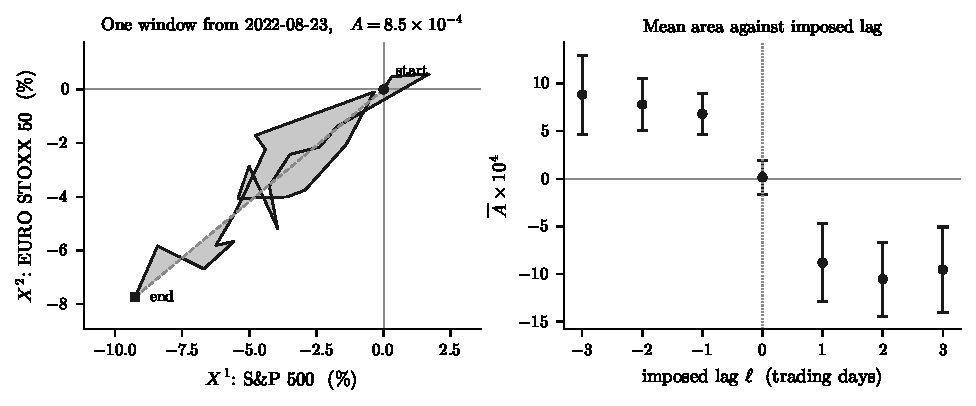
\includegraphics[width=\textwidth]{Images/levy-lag.pdf}
\caption[The L\'evy area and the lag scan]{Left: one monthly window drawn as a path in the plane of
the two cumulative log-returns, with the chord joining its endpoints dashed. The L\'evy area
$A_{0,\Mat}$ is the shaded signed area between path and chord; the endpoints alone fix
$\Sym\lev_{0,\Mat}$ and say nothing about it, which is Proposition \ref{prop:leveltwofree}. Right:
the mean area over $135$ such windows as a function of an imposed lag $\ell$, with $\pm2$ standard
errors. The response reverses in sign with $\ell$ though it is not exactly odd in magnitude, is
detected at more than four standard errors at every non-zero lag, and crosses zero at $\ell=0$
alone.}
\label{fig:levylag}
\end{figure}

The scan behaves as expected; Figure \ref{fig:levylag} draws it. Every non-zero lag is detected at
$|t|\ge4.26$; the area reverses with the imposed lag --- negative under the convention above, in
which a positive $\ell$ makes the first index lead, and positive under the reverse --- so the
statistic reports not only that the series are misaligned but \emph{which} of them leads; and the
zero crossing sits at $\ell=0$ and nowhere else.

% ---------------------------------------------------------------------------
\subsection{The classical route, and why it agrees}
\label{subsec:levyxcorr}

A null area on data whose two exchanges close four and a half hours apart invites one objection
above all others, and it is answered by computing the statistic the area is supposed to improve
upon. Write $\delta^{i}_{t}$ for the daily increments and
$\gamma(h) := \E[\delta^{1}_{t}\delta^{2}_{t+h}]$ for their cross-covariance, with $h>0$ meaning
that the first index leads. For a linearly interpolated pair the level-two entries are
$\lev^{12}=\sum_{i<j}\delta^{1}_{i}\delta^{2}_{j}$ and
$\lev^{21}=\sum_{i<j}\delta^{2}_{i}\delta^{1}_{j}$, so that under stationarity
\begin{equation}\label{eq:areafromxcov}
  \E\bigl[A_{0,\Mat}\bigr] \;=\; \tfrac12\sum_{h=1}^{n-1}(n-h)\bigl[\gamma(h)-\gamma(-h)\bigr].
\end{equation}
The contemporaneous term $\gamma(0)$ is absent: only the \emph{antisymmetric} part of the
cross-covariance survives, which is Remark \ref{rem:rhocancels} read on data rather than on a model.

Both sides of \eqref{eq:areafromxcov} can be measured, and Table \ref{tab:levyxcorr} does so.

\begin{table}[H]
\centering
\small
\begin{tabular}{rrrr}
\hline
$h$ & $\gamma(h)$ & $\mathrm{corr}$ & $t$\\
\hline
$-2$ & $+1.322\times10^{-5}$ & $+0.097$ & $+5.16$\\
$-1$ & $-6.367\times10^{-6}$ & $-0.047$ & $-2.48$\\
$\phantom{-}0$ & $+7.669\times10^{-5}$ & $+0.561$ & $+29.91$\\
$+1$ & $+1.919\times10^{-5}$ & $+0.140$ & $+7.48$\\
$+2$ & $-1.862\times10^{-6}$ & $-0.014$ & $-0.73$\\
\hline
\end{tabular}
\caption[Cross-correlogram of the daily increments]{Cross-correlogram of the daily increments, $2848$ of them, with the Bartlett standard
error $N^{-1/2}=0.019$. The lag-one entry is positive and strongly significant: the first index does
lead the second by a day, exactly as the difference in closing times predicts.}
\label{tab:levyxcorr}
\end{table}

The lag-one effect is therefore real, and large. Taken alone it would put
$\tfrac12(n-1)[\gamma(1)-\gamma(-1)] = 2.56\times10^{-4}$ into \eqref{eq:areafromxcov}, some three
standard errors above what the area measures. What removes it is the rest of the sum. The lag-two
entry carries the opposite sign --- $\gamma(-2)$ is positive and significant while $\gamma(2)$ is
not --- and contributes $-1.43\times10^{-4}$; the remaining lags continue to cancel, and the full
sum \eqref{eq:areafromxcov} comes to $2.99\times10^{-5}$ against a measured
$\overline{A}=1.52\times10^{-5}$. The two routes agree to $0.17$ standard errors.

That is the resolution, and it is worth stating in the order the evidence arrives. The
non-synchronous closing effect is present in the data and the correlogram finds it at $t=+7.5$. The
area does not contradict that reading; it reports the $(n-h)$-weighted antisymmetric \emph{sum} over
all lags, in which the one-day lead is very nearly cancelled by what follows it. A cross-correlogram
scanned lag by lag would have stopped at the first entry and concluded that the pair is
misaligned. Whether the net is the quantity one wants is a modelling decision and not a statistical
one --- but the two statistics are measuring what they claim to, and on this pair they agree. 

% The estimator is not blind. It reports zero on the synchronous data
% because the synchronous data has no lead--lag to report.

% Two robustness checks close the argument, both aimed at the possibility that a handful of extreme
% windows is doing the work.

% \begin{itemize}
%   \item \emph{Trimming.} Discarding the $5\%$ of windows with the largest $|A|$ moves the synchronous
%     statistic from $t=+0.17$ to $t=+0.89$: still null. On the $\ell=+1$ control the same trimming
%     moves $t=-4.31$ to $t=-7.65$, that is, the effect \emph{strengthens} when the outliers are
%     removed. A crisis-driven artefact behaves in the opposite way.
%   \item \emph{Circular block bootstrap} of the mean, with block length $\lfloor\sqrt{M}\rfloor$ to
%     preserve serial dependence across windows. The synchronous $95\%$ interval is
%     $[-1.21,+1.45]\times10^{-4}$ and contains zero; the $\ell=+1$ interval is
%     $[-1.38,-0.52]\times10^{-3}$ and excludes it.
% \end{itemize}

% ---------------------------------------------------------------------------
% \subsection{What the experiment establishes}
% \label{subsec:levyconclusion}

Three comments, of decreasing generality.

\emph{The level-two object is computable and its algebra is exact.}  Chen's relation, geometricity
and the invariance of the area under the choice of stochastic integral hold identically for any
piecewise-linear path, so reproducing them to rounding error on eleven years of real closes tests
the implementation rather than the market --- which is precisely what one wants of them before any
inference is drawn. 

\emph{The area is a signed, calibrated detector of lead--lag, and it measures something a
correlation cannot.} Table \ref{tab:levylag} exhibits an instrument that is null at alignment,
grows with misalignment and reports direction through its sign. Remark \ref{rem:rhocancels} explains
why this is not a repackaged correlation: in the model \eqref{eq:leadlagmodel} the contemporaneous
coupling $\rho$ and the lagged coupling $\leadlag$ are separately adjustable, and the area is exactly
blind to the first. The symmetric part of the tensor, which on this pair is some fifty times larger,
is where the correlation lives. The two statistics are measurements of orthogonal components of one
object, and Proposition \ref{prop:leveltwofree} is the statement that between them they exhaust it.

\emph{On this pair, at daily frequency, the area does not detect a lead--lag.} That is a failure to
reject rather than a demonstration of absence, and it should be recorded as such. What the
calibration adds is that the instrument is not simply blind: the same statistic that returns
$t=0.17$ here returns $|t|>4$ against a one-day displacement of the same data. A displacement of a
whole day is, however, a very large signal, and the scan says nothing about power against a
realistic one. The natural objection --- that the S\&P and the EURO STOXX close some four and a half
hours apart, which is manifestly a lead--lag --- is answered in \S\ref{subsec:levyxcorr} rather than
dismissed: the effect is in the data, the correlogram finds it at $t=+7.5$, and the area is null
because the one-day lead is cancelled by the lags behind it, not because the statistic cannot see
it. What remains is a limitation of the sampling rather than of the estimator. A displacement
shorter than the interval does not leave the expected area unchanged: for two-sided Brownian drivers
observed at unit spacing with an offset $\delta\in(0,1)$, the linearly interpolated pair has
$\E[A]=\delta/2$ rather than $0$, because the overlap of the two increments contributes $\delta$ to
one cross-covariance and nothing to the other. A sub-daily offset is therefore invisible to both
statistics alike, and resolving it requires intraday sampling, at which point the offset moves
inside the observable range. 


% ===========================================================================
% \section{Calibration to Single Names: De-Americanisation}\label{sec:deamericanisation}

% The local volatility surface of Subsection \ref{subsec:localvol} was constructed from European
% quotes, as was the implied volatility surface of Section \ref{sec:pinn}. Single-name options are
% American, and bridging that gap is the first practical step in any calibration on individual
% equities. This section carries out the procedure deferred in Chapter \ref{ch:finance}.

% A major practical hurdle arises during calibration: Dupire's formula (Theorem \ref{thm:dupire})
% requires the partial derivatives of \emph{European} option prices, but single-name market quotes are
% American. We cannot apply Dupire directly to American prices.

% Therefore, calibrating the local volatility surface to American options requires a short, iterative
% mapping procedure known as \textbf{De-Americanisation}:
% \begin{enumerate}
%     \item \textbf{Quote Extraction:} Obtain the market prices of the liquid American options and
%     calculate their Black--Scholes implied volatilities using an American pricer (such as a Binomial
%     Tree or a PDE solver).
%     \item \textbf{Pseudo-European Mapping:} Assume these implied volatilities approximate the
%     volatilities of European options with the exact same strikes and maturities. Use these
%     volatilities to generate a grid of ``pseudo-European'' option prices.
%     \item \textbf{Local Volatility Construction:} Apply a smoothing parameterisation to the
%     pseudo-European surface to ensure it is free of static arbitrage --- either SVI
%     \cite{gatheral2014} or the arbitrage-penalised surface of Section \ref{sec:pinn} --- and then
%     apply Gatheral's form \eqref{eq:gatheral} of the Dupire formula to construct the local volatility
%     surface $\lvol(\lmon,T)$.
%     \item \textbf{Repricing and Verification:} Substitute this $\lvol$ back into the LCP
%     (Equation \eqref{eq:LCP_American}) and solve it backwards using a finite difference method (such
%     as Crank--Nicolson combined with a Projected Successive Over-Relaxation (PSOR) algorithm) to
%     verify that the model accurately recovers the original American market quotes.
% \end{enumerate}

% This iterative procedure effectively bridges the theoretical gap between the European foundations of
% Local Volatility and the practical reality of American single-name markets, ensuring that our models
% reflect true market dynamics without introducing arbitrage.

% Step 3 is where Section \ref{sec:pinn} enters. The de-Americanisation loop needs a surface that is
% arbitrage-free \emph{and} differentiable twice in $\lmon$ and once in $T$, since
% \eqref{eq:gatheralrecall} is evaluated on it; and it needs that surface to be defined beyond the
% quoted range, because a single-name book carries far fewer strikes than an index and the PDE solve of
% step 4 requires boundary data well outside them. Those are exactly the two properties that
% \eqref{eq:surface} was built to have.

% \section{Implementation}
% \label{sec:implementation}

% \section{Results}
% \label{sec:results}

% \subsection{Index books}
%
% On a liquid index book the calibration is comfortable. A representative date
% carrying $3048$ grouped quotes across $18$ maturities returns a mean absolute
% distance to mid of $4.5$ basis points, an $80$th percentile of $6.7$, and zero
% butterfly and zero calendar violations on an independent scan of half a million
% points. The minimum density sits on its imposed floor, no node is rescued by
% curvature, and no trusted quote pair moves the wrong way.
%
% The residual disagreement is concentrated at the money and is not a modelling
% failure: the put/call gap on that date reaches fifteen half-spreads, and the
% in-band fit percentage near $\lmon=0$ is capped by the data's own inconsistency
% rather than by the surface.
%
% \subsection{Single names}
%
% Single-name books are harder, and instructively so. The failures are of two
% kinds.
%
% \emph{Wing failures} are as described above and are now understood: they are
% driven by the interior minimum of $\Caldrift$, whose depth scales with the wing's lift
% $|b|$ and with the maturity drift of the saturation length. Single-name wings
% carry lifts several times larger than index wings, which is why they leak first
% and why they leak on the side with the larger lift.
%
% \emph{Term-structure failures} are a different matter and are not yet solved.

\section*{Notes and references}
\addcontentsline{toc}{section}{Notes and references}

\noindent
The physics-informed neural network methodology is due to Raissi, Perdikaris and Karniadakis
\cite{raissi2019}; the survey \cite{karniadakis2021} places it in the wider setting of
physics-informed machine learning and is the natural entry point for a reader meeting these methods
for the first time. The exactness of the derivatives on which \S\ref{subsec:network} and
\S\ref{subsec:objective} rely is a property of automatic differentiation rather than of neural
networks, and the standard reference is the survey of Baydin et al.\ \cite{baydin2018}. The optimiser
is AdamW \cite{loshchilov2019} with the warm-restart schedule of \cite{loshchilov2017}.

On the financial side nothing in this section is new: the two conditions imposed are those of
Proposition \ref{prop:staticarbitrage}, which is Gatheral's \cite{gatheral2006}, the wing bound is
Lee's \cite{lee2004}, and the local volatility recovered from the fitted surface is Dupire's
\cite{dupire1994} in the implied-variance coordinates of \cite{gatheral2014}. What is new here is the
route: the conditions are imposed as penalties on a globally smooth representation rather than
inherited from a parametric slice family, and on the extrapolated wings they are established as
Lemma \ref{lem:master} and Theorem \ref{thm:wingreduction} rather than sampled.

\medskip

\noindent
Section \ref{sec:roughcalib} rests on the characteristic function of El Euch and Rosenbaum
\cite{eleucrosenbaum2019}, quoted as Theorem \ref{thm:roughhestoncf}; the wider rough volatility
programme in which it sits is surveyed in \cite{bayerfrizfukasawa2023} and \cite{dinunno2023}. The
Fourier route from a characteristic function to a price was opened by \cite{carrmadan1999}; the
form used here, evaluated on the contour $\operatorname{Im}u=-\tfrac12$, is Lewis'
\cite{lewis2001}. The claim that
the at-the-money skew behaves as $T^{\Hurst-1/2}$, on which \S\ref{subsec:rhidentification} turns, is
from \cite{gatheraljaissonrosenbaum2018}. Proposition \ref{prop:noquadrature} is elementary and is
recorded only because it removes the singular quadrature that a direct reading of
\eqref{eq:roughhestoncf} appears to require; the stability cut \eqref{eq:ustab} is likewise a
practical observation rather than a result. The negative conclusion of
\S\ref{subsec:rhidentification} --- that a surface beginning at $38$ days does not identify $\Hurst$,
because the estimator that would do so has no power outside its asymptotic regime --- is, as far as
the author is aware, not stated in this form in the literature, though the weakness of $\Hurst$ under
option-based calibration is known folklore.

\medskip

\noindent
Section \ref{sec:levyresults} draws its theory entirely from Chapter \ref{ch:roughpaths}: the three
identities verified there are Propositions \ref{prop:leveltwofree}, \ref{prop:chenarea} and Remark
\ref{rem:areaconventions}, the model measured is Definition \ref{def:leadlag}, and the estimator is
Proposition \ref{prop:leadlagarea}. The classical route to the same question is a cross-correlogram
scanned over a grid of lags, and what \eqref{eq:leadlagarea} offers against it is recorded in Remark
\ref{rem:rhocancels}: one number in place of a scan, at the cost of committing to the shape of the
model. For the use of signatures as market statistics more generally --- of which the level-two
reading performed here is the smallest instance --- see \cite{lyonsnejadperez2020},
\cite{abijaber2024} and \cite{cuchiero2025}; the references for the transform itself are collected in
the notes to Chapter \ref{ch:roughpaths}.
